\documentclass[usenatbib,usegraphicx,letterpaper]{mn2e}
\usepackage[totalwidth=480pt,totalheight=680pt]{geometry}

\usepackage{amssymb}
\usepackage{epsfig}
\usepackage{amsmath}
\usepackage{color}
\usepackage[dvipsnames]{xcolor}
\usepackage{epsfig}  
\usepackage{graphicx}
\usepackage{subfig}
\usepackage{rotating}
%%\usepackage{physics}

%Journals
\def\pasj{{PASJ}}
\def\nat{{ Nature }}
\def\aap{{ Astron. \& Astrophys. }}
\def\aj{{ Astron.~J. }}
\def\apj{{ Astrophys.~J. }}
\def\araa{{ Ann. Rev. Astron. Astrophys. }}
\def\apjl{{ Astrophys.~J.~Letters }}
\def\apjs{{ Astrophys.~J.~Suppl. }}
\def\apss{{ Astrophys.~Space~Sci. }}
\def\icarus{{ Icarus }}
\def\mnras{{ MNRAS }}
\def\pasp{{ Pub. Astron. Soc. Pacific }}
\def\planss{{ Plan. Space Sci. }}
\def\physrep{{ Phys. Rep.}}
\def\jcap{{J. Cosm. Astropart. Phys.}}

% less then similar, greater than similar
\def\lsim{\lower0.6ex\vbox{\hbox{$ \buildrel{\textstyle <}\over{\sim}\ $}}}
\def\gsim{\lower0.6ex\vbox{\hbox{$ \buildrel{\textstyle >}\over{\sim}\ $}}}

% begin equation
\newcommand{\beq}{\begin{equation}}
\newcommand{\eeq}{\end{equation}}
\newcommand{\beqa}{\begin{eqnarray}}
\newcommand{\eeqa}{\end{eqnarray}}

% basic cosmology
\newcommand{\Ho}{H_{0}}
\newcommand{\Om}{\Omega_{\mathrm{M}}}
\newcommand{\Ol}{\Omega_{\Lambda}}
\newcommand{\Ode}{\Omega_{\mathrm{DE}}}
\newcommand{\rhocrit}{\rho_{\mathrm{crit}}}
\newcommand{\Ok}{\Omega_{\mathrm{K}}}
\newcommand{\wzero}{w_{0}}
\newcommand{\wa}{w_{\mathrm{a}}}
\newcommand{\wpiv}{w_{\mathrm{piv}}}
\newcommand{\apiv}{a_{\mathrm{piv}}}
\newcommand{\ellmax}{\ell_{\mathrm{max}}}
\newcommand{\fsky}{f_{\mathrm{sky}}}

\newcommand{\fom}{\mathcal{F}}
\newcommand{\Rvir}{r_{\mathrm{vir}}}
\newcommand{\Rdel}{r_{\Delta}}

% units
\newcommand{\Msun}{\mathrm{M}_{\odot}~}
\newcommand{\hMsun}{\ h^{-1}\mathrm{M}_{\odot}~}
\newcommand{\hMpc}{\ h^{-1}\mathrm{Mpc}~}
\newcommand{\hkpc}{\ h^{-1}\mathrm{kpc}~}
\newcommand{\cpiv}{c_{\mathrm{piv}}}
\newcommand{\kmsmpc}{~\mathrm{km/s/Mpc}~}
\newcommand{\kms}{~\mathrm{km}~\mathrm{s}^{-1}}
\newcommand{\Mpc}{\mathrm{Mpc}}
\newcommand{\kpc}{\mathrm{kpc}}
\newcommand{\pc}{\mathrm{pc}}
\newcommand{\au}{\mathrm{AU}}
\newcommand{\gev}{\mathrm{GeV}}

% roman differential
%\newcommand{\dd}{\mathrm{d}}

% comments
\newcommand{\arz}[1]{{\color{BrickRed}\textbf{ARZ:}\textbf{#1}}}


\bibliographystyle{mn2e}

%%%%%%%%%%%%%%%%%%%%%%%%%%%%%%%%%%%%%%%%%%%%%%%%

\begin{document}

\title[Halo Environmental Effects as a Function of Halo Definition]{Halo Definition and Environmental Effects}
\author[Antonio Villarreal, Andrew R. Zentner, Christopher W. Purcell]
{Antonio Villarreal$^1$\thanks{E-mail: asv13@pitt.edu},
 Andrew R. Zentner$^1$\thanks{E-mail: zentner@pitt.edu}, 
 Christopher W. Purcell$^2$\thanks{E-mail: cwpurcell@mail.wvu.edu}\\
$^{1}$Department of Physics and Astronomy \& \\
Pittsburgh Particle Physics, Astrophysics, and Cosmology Center (Pitt-PACC),\\ 
University of Pittsburgh, Pittsburgh, PA\\
$^{2}$Department of Physics and Astronomy, \\
West Virginia University, Morgantown, WV}

\date{In preparation}

%%\pagerange{\pageref{firstpage}--\pageref{lastpage}} \pubyear{2015}

%% \label{firstpage}

\maketitle

\begin{abstract}
%% Abstract goes here
Recent work has shown the importance of environment to the properties of dark matter halos. This brings conflict to standard implementations of the halo model and excursion set theory which assume that the properties of a population within the halo is determined by the mass of the halo alone. We seek to find a definition of the size of a halo that allows us to circumvent these environmental effects. We analyze the dependence on environment of our properties using the method of marked correlation functions for several different halo definitions, utilizing the Consuelo and Diemer et al simulations. We find that environmental dependencies are dramatically different as we vary the definition of the halo radius in terms of the overdensity parameter $\Delta$.  Further, we analyze the mass dependence on these effects and how they factor into the ultimate applicability of our methodology.
\end{abstract}

\begin{keywords}
dark matter -- galaxies: halos -- galaxies: formation -- large-scale structure of universe -- methods: numerical
\end{keywords}

%% notes on citation style:
%% \citep{stuff01,stuff02,stuff03} produces (Stuff 2001; Stuff 2002; Stuff 2003)
%% \citet{stuff04} produces "Stuff (2004)" in the main body
%% \\* defines a break in a section title it appears?
%% \begin{enumerate} into \item allows you to do the (i), (ii), (iii) thing 

%-----------------------
\section{Introduction}
\label{section:introduction}
%-----------------------

 \arz{We will need to work on the introduction considerably as we get a better handle on the final results. The first two paragraphs can probably be 
 combined into a single shorter paragraph. I also like to end the first paragraph by telling the reader what it is that we aim to do in the paper.}

In the current concordance cosmology, the creation of observed galaxies and clusters is often seen as arising from the hierarchical mergers of dark matter halos.\citep{white78}. Being able to model the properties of dark matter halos and the galaxies within gives us a potential probe for the physical processes that go into galaxy formation. The excursion-set formalism of galaxy clustering \citep{bond91,lacey93,somerville99, zentner06} and the standard halo model of galaxy clustering \citep{seljak00, peacock00, scoccimarro01, berlind02, bullock02, cooray02} both can help us in this task, but rely on underlying asumptions. The first is that the statistics of the objects within a dark matter halo is a function of the mass alone. The second is that the clustering of dark matter halos is a function of mass as well. In this paper we propose a simple redefinition of halo size that will help correct for inaccuracies in these two assumptions.

It has previously been demonstrated that the clustering of halos is dependent on not only dependent on the mass, but also on the formation time of the halo \citep{sheth04, gao05, croton07}. Furthermore, it has been shown that the clustering of a given halo is dependent on the halo concentration \citep{wechsler06}. This necessitates corrections be made to the standard implementations to account for this. More complicated methodologies have been made to extend to using merger histories directly from simulation \citep{dvorkin11}, as well as to account for the dependence due to concentration \citep{gil11}. The relationship that clustering has to the properties of the halo can be described as environmental effects.

Our method of halo redefinition is motivated by the size of a halo being an ill-defined quantity. What if often referred to as the ``virial radius'' will not contain all gravitational bound dark matter particles in the halo \citep{kazan06}. Rather, it is a matter of convention that does not have a common definition. We choose to define a halo radius in a way that encompasses the nearby environmental effects. These may be due to large scale structure or driven by baryonic physics. Using a simulated box, we can then test how the redefinition of the halo size affects the relationship between the clustering and the properties of the halo. In the case that the properties of the halo become independent of the clustering, it is possible to utilize standard implementations of the halo model without necessitating more complicated theory.
 
In \S~\ref{section:data} of this paper, we consider the simulated cosmological boxes that we utilize for our statistics and our method of halo size redefinition. In \S~\ref{section:methodology}, we discuss the statistics that we have used in order to test for environmental effects and the removal of known mass scaling from these statistics. In \S~\ref{section:results}, we present our results on our tests and draw conclusions as to the natures of the encountered environmental effects. In \S~\ref{section:conclusions}, we discuss the significance of redefining environmental effects through a redefinition of halo environments and discuss possible applications of our methodology.

%------------------------------------
\section[]{Simulation Data and Halo Finding}
\label{section:data}
%------------------------------------

In order to study the effects of halo redefinition, we make extensive use of two simulation suites. The Diemer et al simulations each utilize a Planck best fit cosmology with $\Om = 0.32$, $\Ol = 0.68$, and $h_o = 0.67$. We use three simulation boxes with comoving sizes of $125, 250, and 500 \hMpc$ respectively. The particle mass of $1.6 \times 10^8 \hMsun$, with a total of $1024^3$ particles in each simulation. This set of simulations allows us to probe the resolution effects on halo finding, as each box has a factor of eight difference in effective resolution. We also analyze the Consuelo simulation from the Large Suite of Dark Matter Simulations (LasDamas) (McBride et al, in prep? I literally cannot find this paper despite it being in prep since 2012!) :which ran with a cosmology with $\Om = 0.25$, $\Ol = 0.75$, and $h_o = 0.7$. This simulation box has a comoving size of $420 \hMpc$ and a particle mass of $1.87\times 10^9 \hMsun$, with a total of $1400^3$ particles. The difference in cosmology between the two sets of boxes will allow us to determine if this has drastic implications on our method.

For halo finding we use the ROCKSTAR halo finder, which works on the phase space algorithm described in \citet*{behroozi13}. In short, ROCKSTAR determines the initial groupings using a FOF algorithm in phase space, before then applying the spherical overdensity case in order to determine the properties of interest. Unbound particles are removed prior to the calculation of halo mass and other properties of interest. In addition, we take interest of the shape of the halo, which is determined through the sorted eigenvalues of the inertia tensor, with principal ellipsoid axes defined such that $a >b > c$. Some of these parameters are determined after fitting the particles to the Navarro-Frenk-White profile \citep*{nfw97}.

Given the nature of the halo size as a hard to define statistic, we choose to redefine the halo in terms of the overdensity parameter, $\Delta$, by defining the halo radius, $\Rdel$, as follows:

\beq
	\rho(\Rdel) = \Delta \rho_b
\eeq

Here, $\rho_b$ is the background mass density of the simulation box, while $\rho$ is the density measured within at a radius under the assumption that it uniformly distributed in a sphere of radius $\Rdel$. It should be noted that the use of the critical density or the mean density is interchanged within the literature, though the change is relatively mild. We allow the overdensity parameter $\Delta$ to vary over the range of the fiducial definition of $\Delta = 200$ down to values as extreme as $\Delta = 10$. As discussed above, this change is motivated due to the fact that the definition of halo size is primarily a matter of convention.

With the combination of this analysis and the ROCKSTAR data, we define the following properties of interest:

\beq
	c_{\mathrm{vratio}} = \frac{v_{\mathrm{max}}}{v_{\Delta}} ; \ \ c_{\mathrm{NFW}} = \frac{\Rdel}{r_\mathrm{s}}; \ \ s = \frac{c}{a}; \\ \Lambda = \frac{J \sqrt{\lvert E\rvert}}{G M_{vir}^{2.5}} \\
\eeq

\begin{figure}
	\centering
		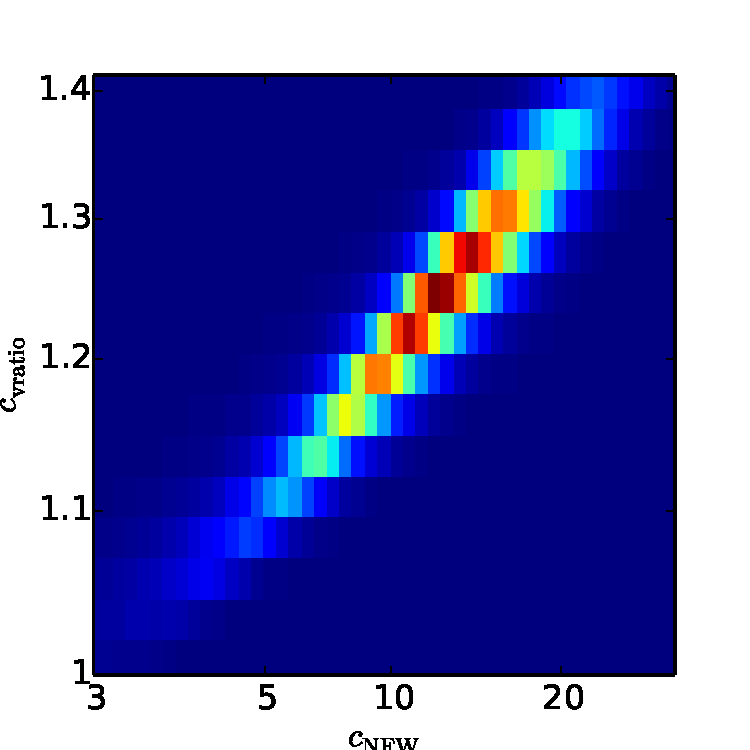
\includegraphics[width=.5\textwidth]{ldcompare_cnfwvscvrat_z00.pdf}
	\caption{The relationship between the two different marks of concentration, using halos in the Consuelo simulation box.}
\end{figure}

The first two marks listed above are different proxies for the concentration of the halo. The relationships between these marks are shown in Figure 1 and it can be seen that they can be related to each other with some scatter. The ROCKSTAR catalogs give us the max  circular velocity of a hypothetical particle, $v_{\mathrm{max}}$, the scale radius, $r_{\mathrm{s}}$, the halo radius, $\Rdel$, both ellipsoidal axis parameters $c$ and $a$, and the spin parameter, $\Lambda$ as introduced by \citep{peebles69} in terms of the halo angular momentrum $J$ and the total energy of the halo $E$ . The circular velocity of a particle at the halo radius is calculated by $v_{\Delta} = \sqrt{\frac{G M(< \Rdel)}{\Rdel}}$.

%-----------------------
\section[]{Methodology}
\label{section:methodology}
%-----------------------

There are several well understood effects in our simulation that must be accounted for before we can draw any conclusions. The first is the matter of simulation resolution. In each of our generated halo catalogs, we can anticipate finding artificial halos. While existing under our constraint of having only a set overdensity, they will have properties that conflict with well known trends that have been shown in prior works, such as concentration decreasing as a function of halo mass \citep{wechsler06}. As shown in Figure 2, we can roughly identify the region in which these artificial halos become significant by looking for the turnover in the plot. In order to avoid our halo finding statistics being thrown off by these artificial halos, we set a lower mass threshold, limiting the sample to only those halos that are physically significant. We choose to use the higher mass constraint between the Max and Consuelo simulation boxes for consistency.

\begin{figure}
	\centering
		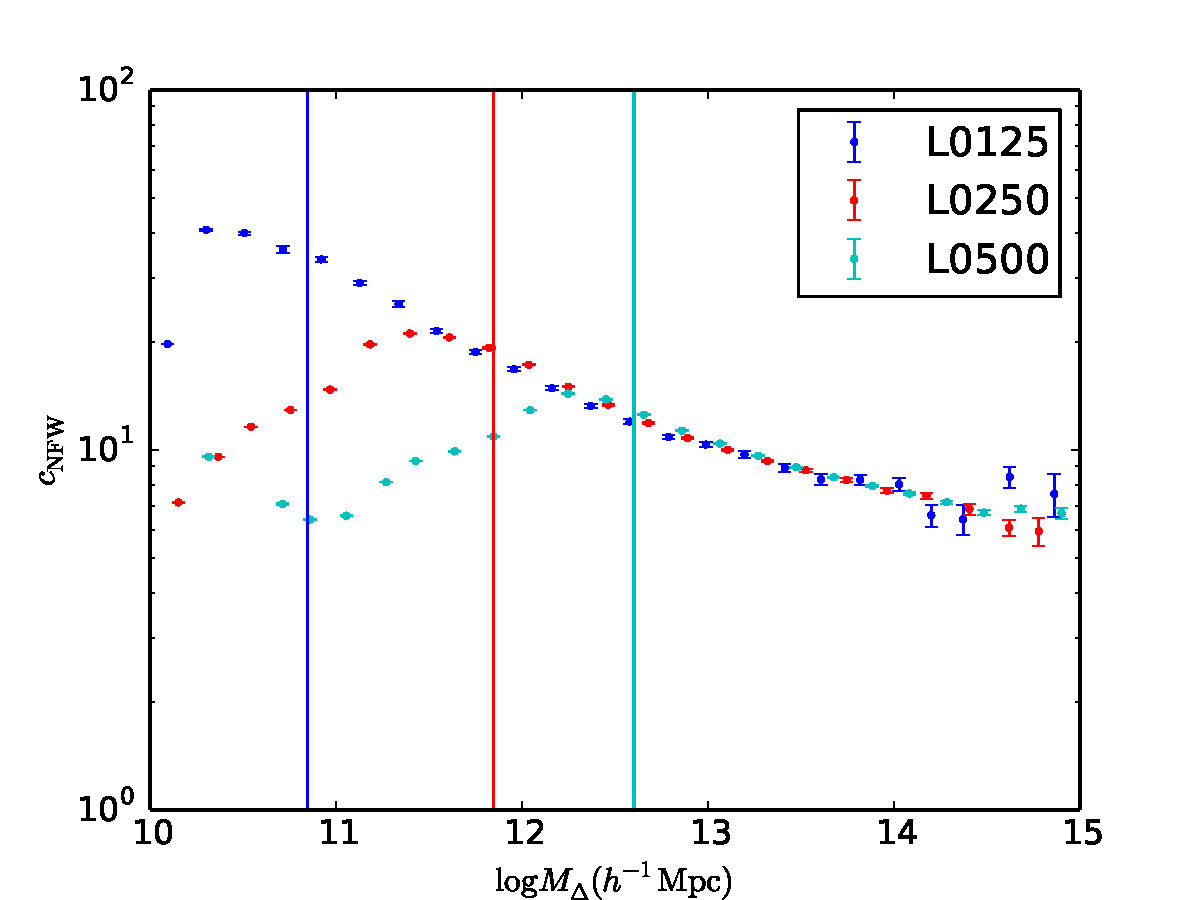
\includegraphics[width=.5\textwidth]{masscut_cnfw_d200.pdf}
	\caption{An example of the chosen lower limit on halo mass for our sample is marked as a black line, for the $\Delta = 200$ case. The shaded blue region depicts the spread on the power in the concentration-mass relationship proposed by \citet{duffy08}.  The shaded region illustrates the implied two-sigma band of \citet{duffy08} mass-concentration relation. At lower mass, halos are ill defined due to resolution limits.}
\end{figure}

Another well known effect is the scaling of our properties as a function of halo mass, as well demonstrated within the literature \citep{duffy08}. We are interested in the clustering behavior beyond this well known effect, so we seek to remove this scaling. We take all host halos of interest and sort them by their halo mass. Each set of halo properties are then placed in bins of equal population in order to assure that enough data points exist for robust statistics. We then normalize each mark in a given bin to the mean value. The end result is halo properties that do not change as a function of mass, allowing us to more accurately analyze clustering behavior within our simulation.

To normalize the satellite number we follow the prescription of \citet{wechsler06}. In addition to the mass cutoffs on our data, we eliminate ill-resolved satellites by choosing a cutoff in $v_{\mathrm{max}}$ for the host halo. We then attempt to match subhalos to this mass halo, making a secondary cutoff in the case that the value of $v_{\mathrm{max,sub}} / v_{\mathrm{max,host}}$ is not above a threshold value. We set these two parameters such that there are no isolated or poorly resolved subhalos in our data sample.

In order to test for environmental effects, we choose to utilize two primary methods. The first is to look at the two-point correlation functions of the host halo catalog and compare it against the correlation functions of the top and bottom 20\% of most concentrated host halos. Assuming that each halo was statistically similar, we would expect that there would be no discernible difference between these correlation functions in the case where there are no environmental effects. We utilize a jackknife method in order to estimate the errors on these correlation functions.

The second method is to use a weighted correlation function, often referred to in the literature as the marked correlation function (MCF). Our marks in this case are the log values of the halo concentration proxies described previously, the halo shape, and the halo satellite number. The use of this tool in measuring clustering has been shown previously in \citet{wechsler06} or \citet{harker06}. We compare our MCFs to an error bar representing the approximate 2-sigma confidence region generated by randomizing the marks among our halos 400 times and taking the 10th lowest and 390th highest values of the mark among the randomizations. In the case of no environmental effects upon the property of interest, one would expect that the MCF would fall within the region bounded by these limits.

%----------------------------
\section[]{Results and Discussion}
\label{section:results}
%----------------------------

%% for the time being, we should seek to have a square grid of plots - L0125, L0250, L0500, and Consuelo, for each major results plot. Time to Google how to do that!
%% also, consider redoing this first plot. Perhaps do xi_highconc / xi_lowconc? Original problem with this was different radial bin centers, but this can be checked against
%% for severity. Shouldn't be too bad an approximation though, and should also be less visually cluttered.
%% perhaps just slap a \\ after the second subfloat and repeat? Maybe?
\begin{figure*}
	\centering
	\subfloat[L0125]{{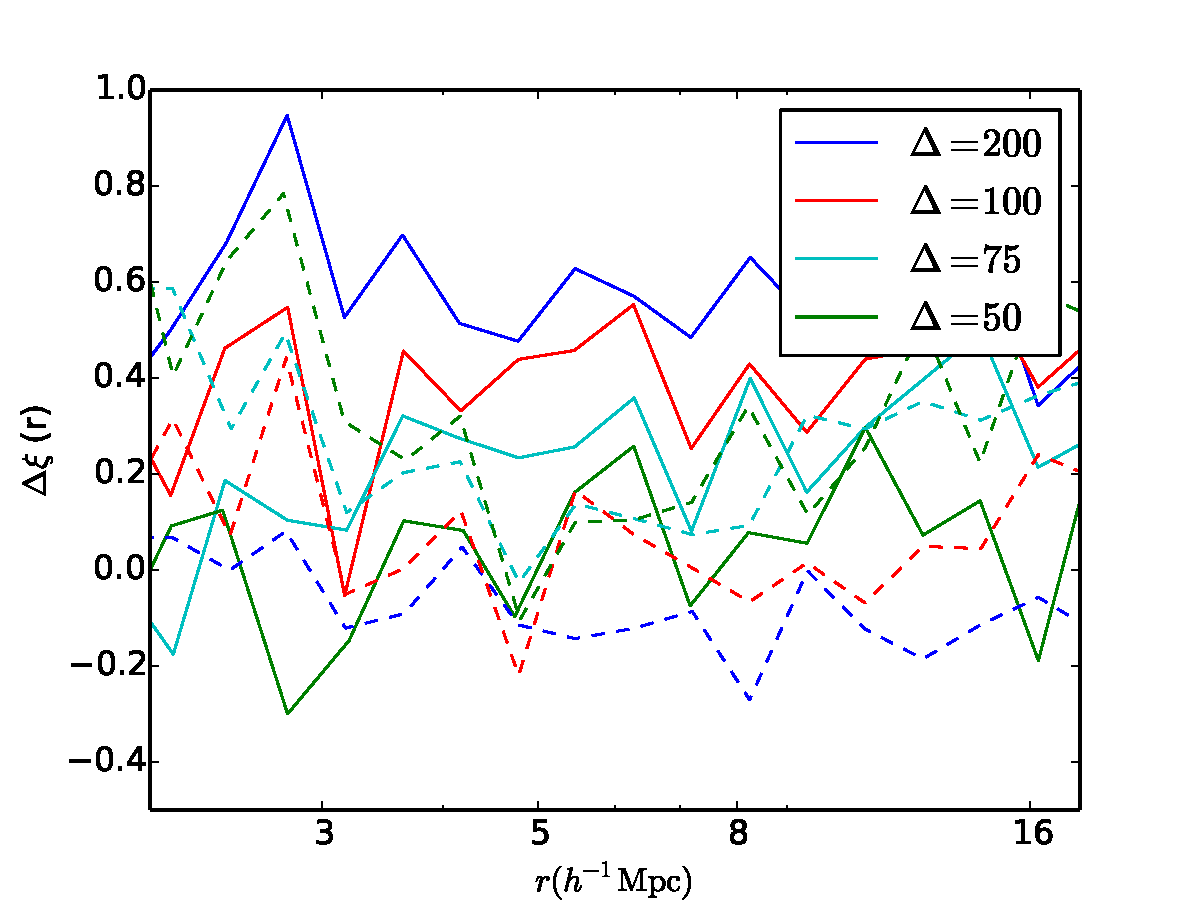
\includegraphics[width=.45\textwidth]{L0125_cf_compare_z00_hosts.pdf}} }
	\subfloat[L0250]{{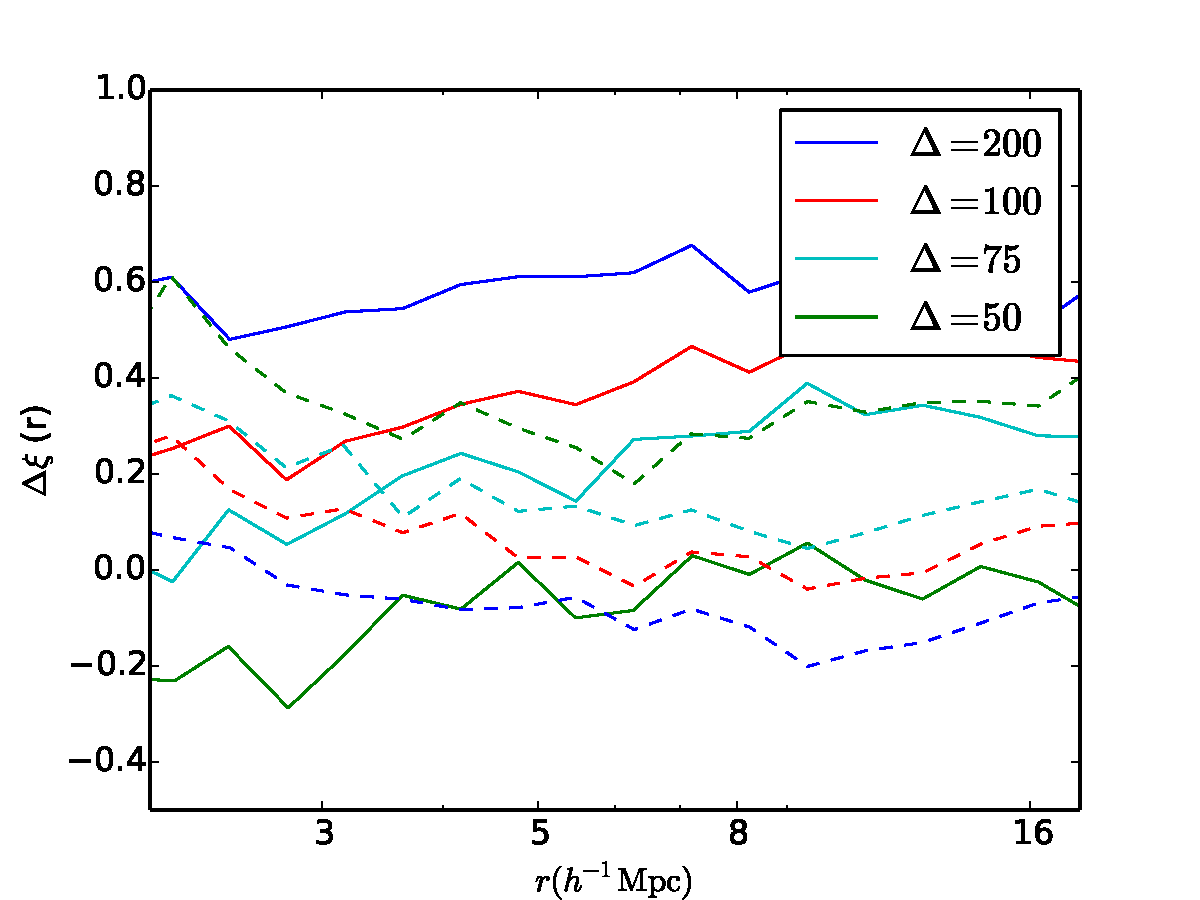
\includegraphics[width=.45\textwidth]{L0250_cf_compare_z00_hosts.pdf}} }
	\\
	\subfloat[L0500]{{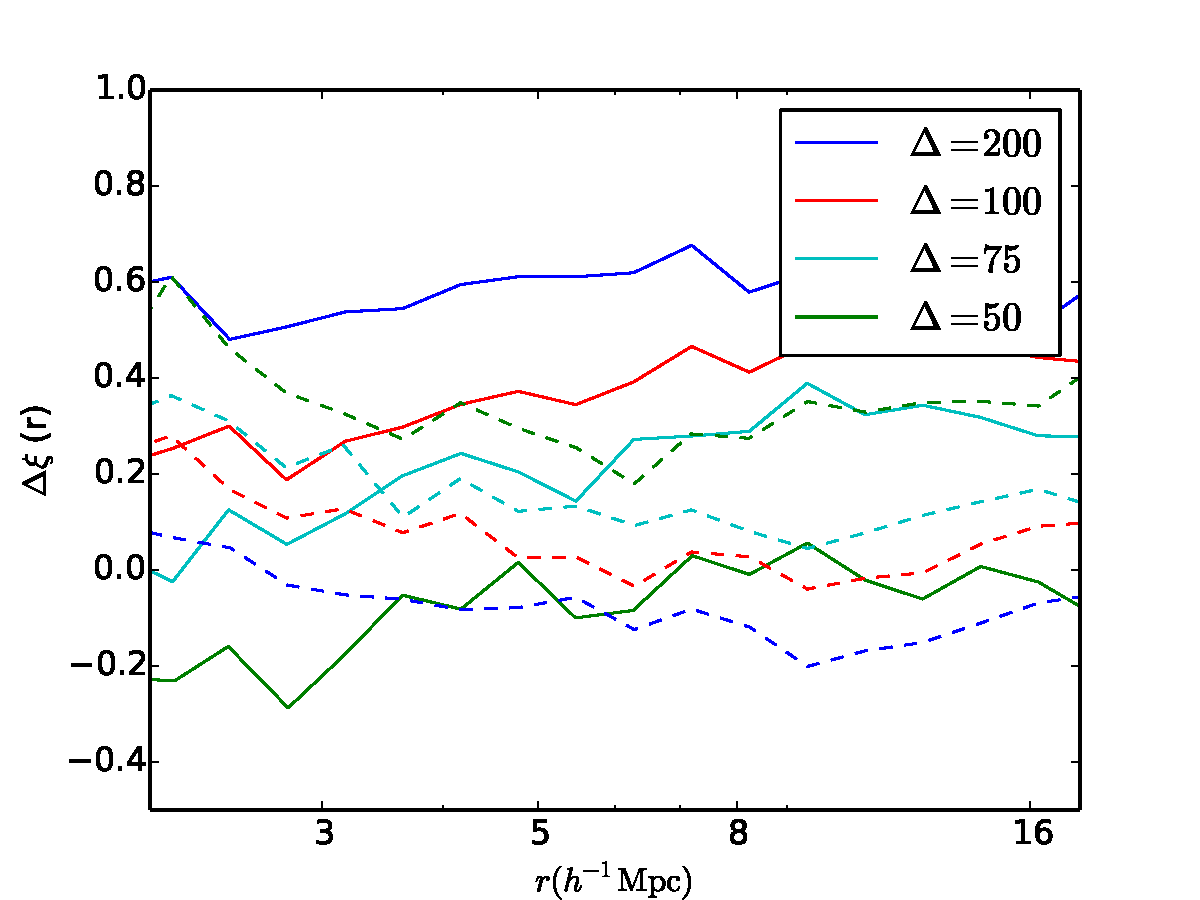
\includegraphics[width=.45\textwidth]{L0250_cf_compare_z00_hosts.pdf}} }
	\subfloat[Consuelo]{{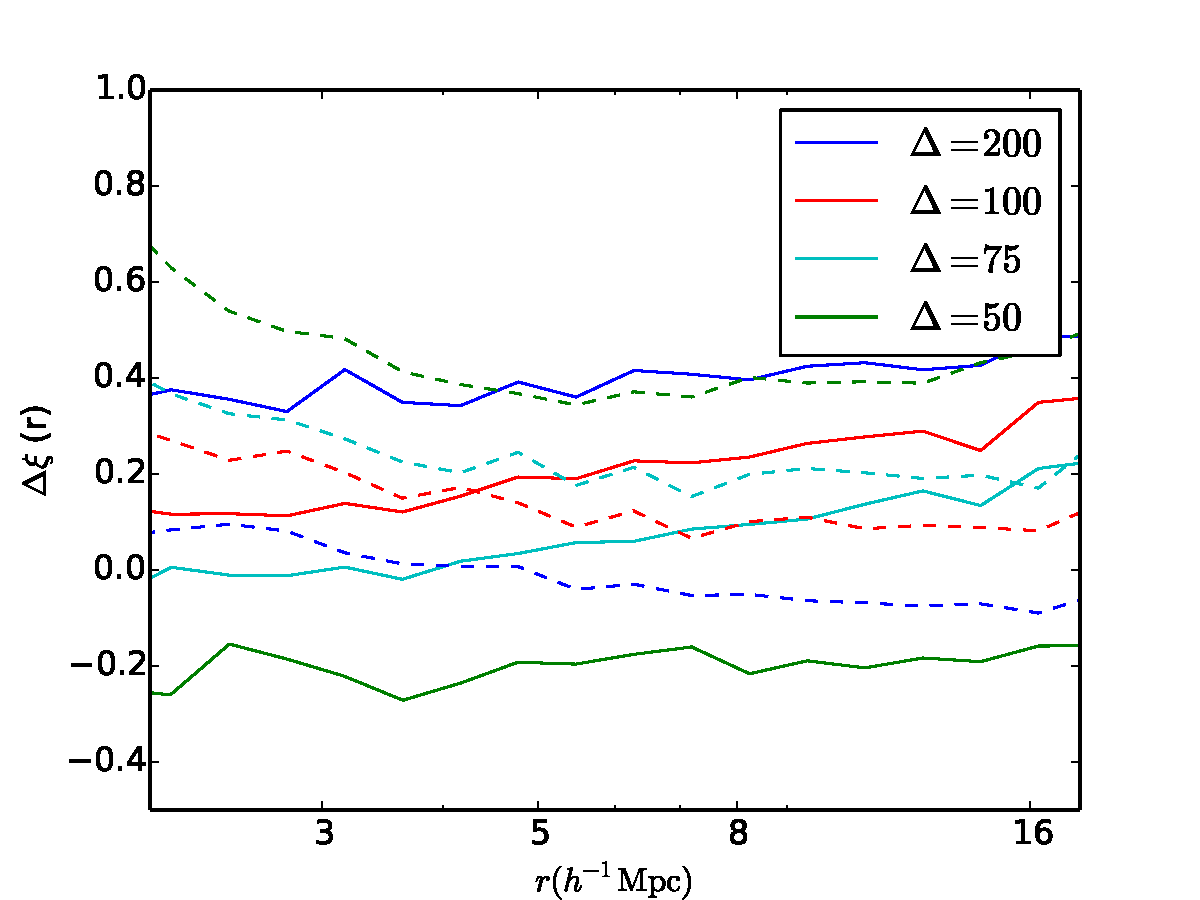
\includegraphics[width=.45\textwidth]{ld_cf_compare_z00_hosts.pdf}} }
	\caption{The difference of the correlation function of all hosts compared to a cut of the 20 \% highest or lowest NFW defined concentration halos. The solid lines represent the difference from the highest concentration cut, the dashed lines represent the difference from the lowest concentration cut.}
\end{figure*}

Figure 3 demonstrates the results of our method as we change the value of $\Delta$. It can be seen that for between the values of $\Delta = 100$ and $\Delta = 75$ that both the high and low concentration cuts of the data can be brought into close agreement. This feature is seen in both the Consuelo and Max simulations. It should be noted that both the high and low concentration cuts move closer toward a state with environmental dependencies being thoroughly removed within the margin of error from opposite directions in terms of clustering. Changing the value of $\Delta$ beyond the observed ``sweet spot" appears to reintroduce the problem we are attempting to remove.

\begin{figure*}
	\centering
	\subfloat[L0125]{{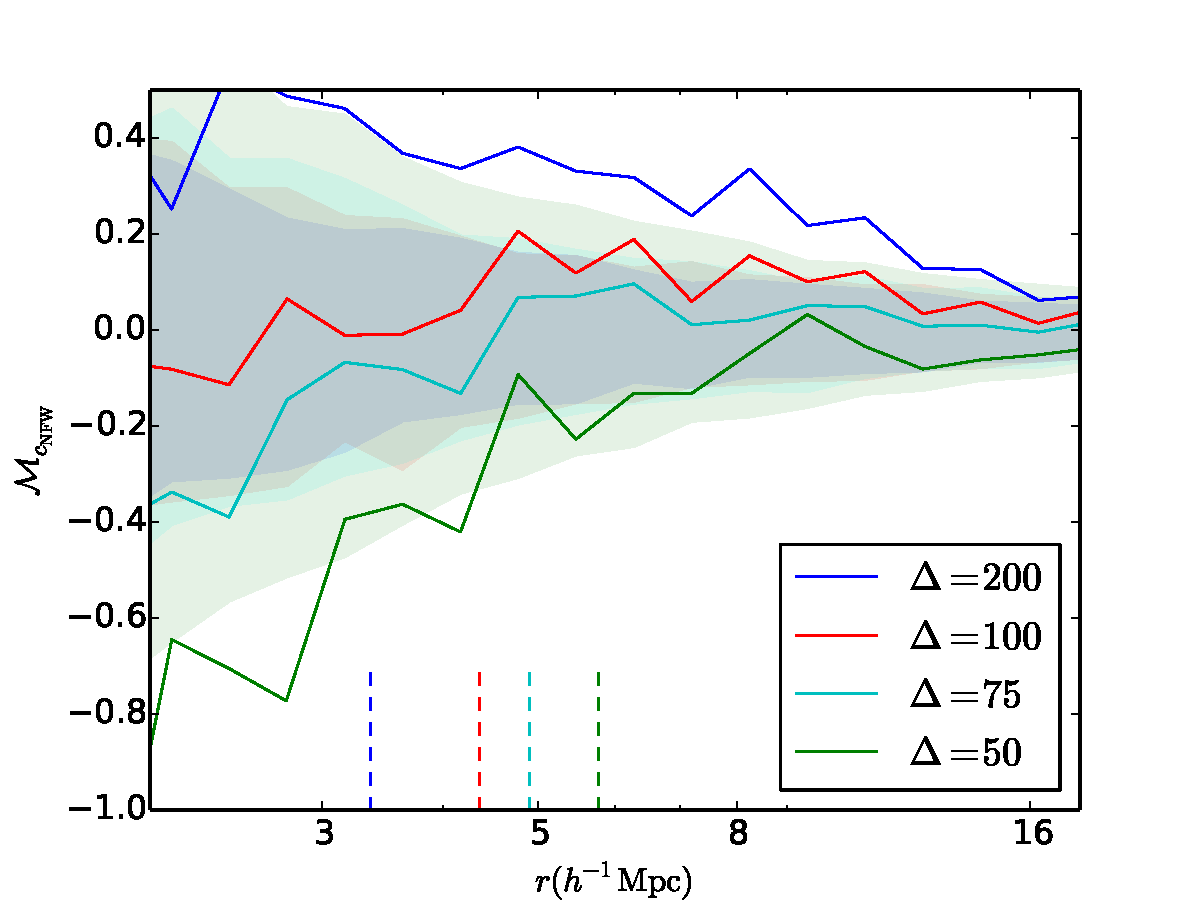
\includegraphics[width=.45\textwidth]{L0125_mcf_cnfw_z00_hosts.pdf}} }
	\subfloat[L0250]{{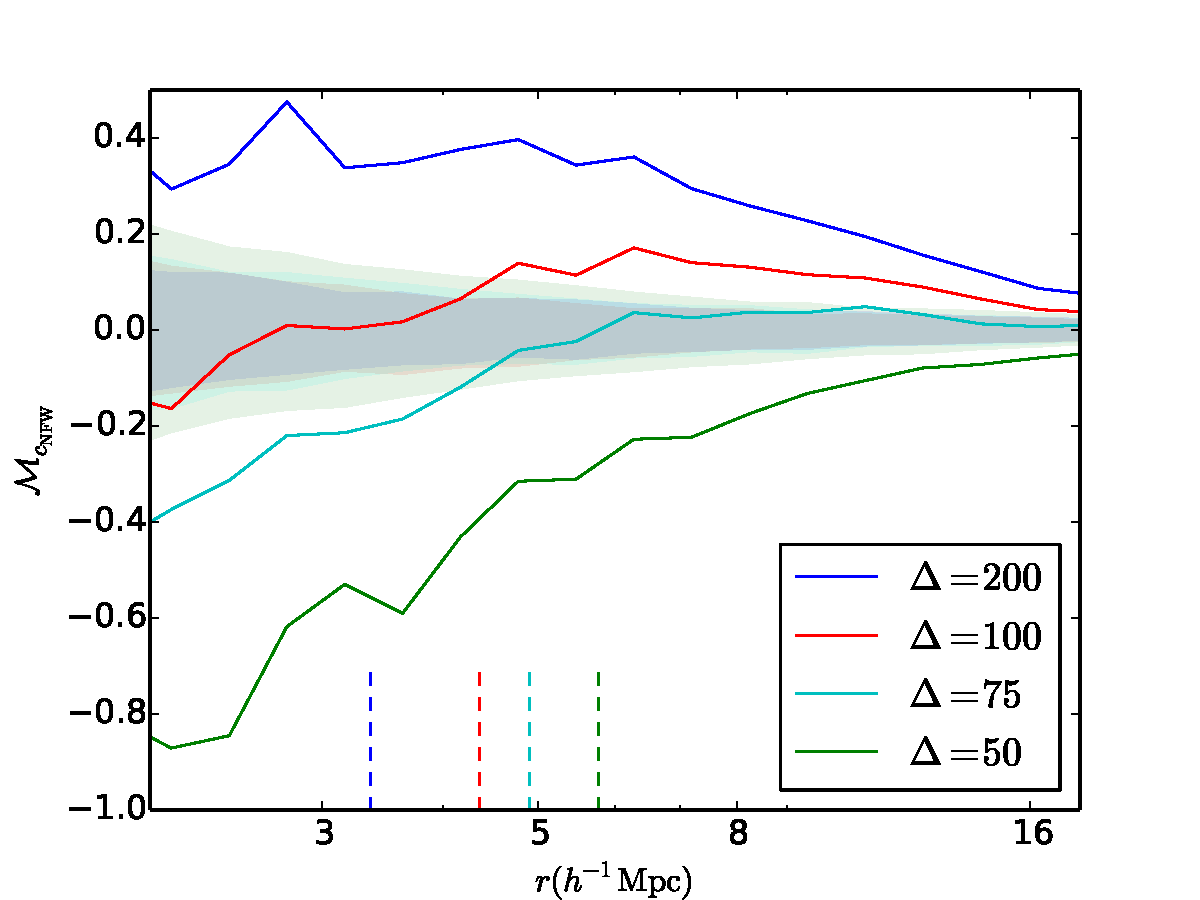
\includegraphics[width=.45\textwidth]{L0250_mcf_cnfw_z00_hosts.pdf}} }
	\\
	\subfloat[L0500]{{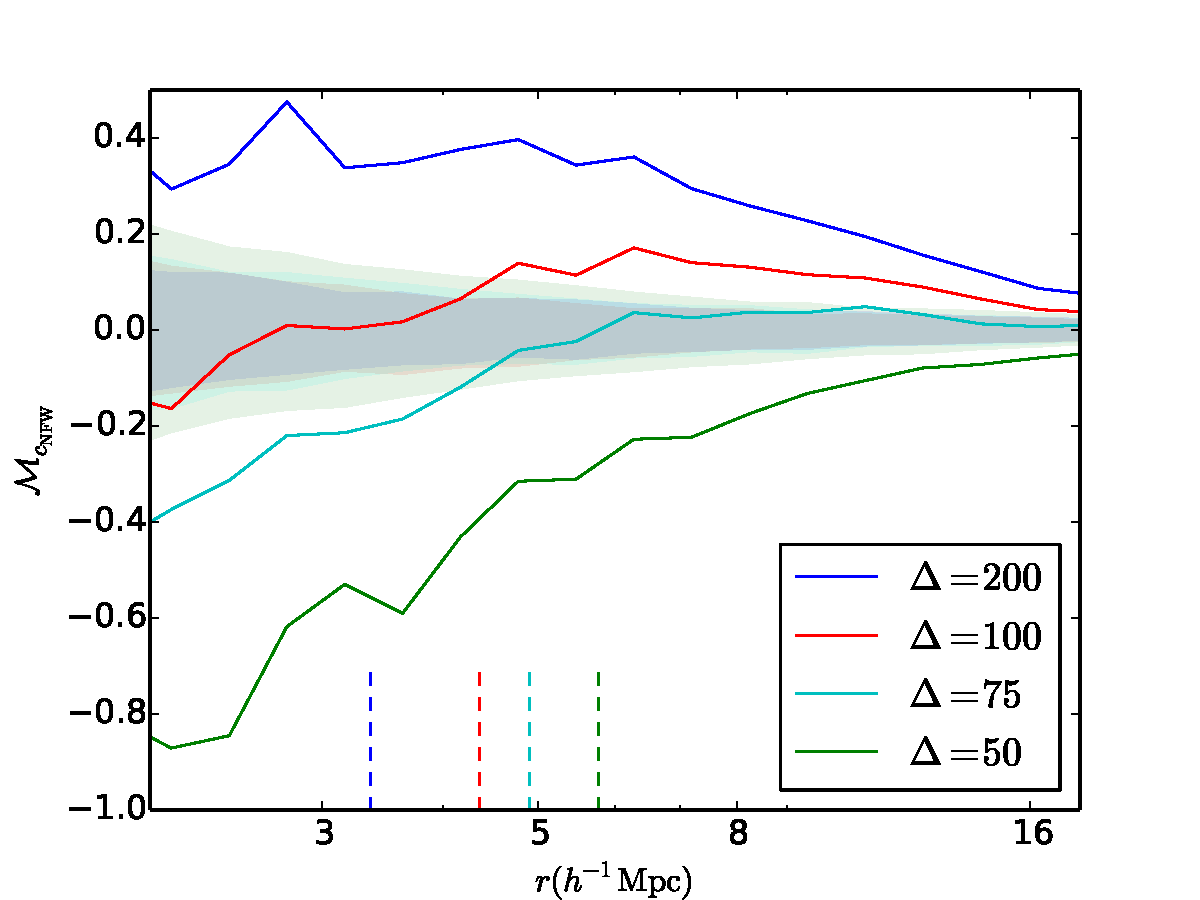
\includegraphics[width=.45\textwidth]{L0250_mcf_cnfw_z00_hosts.pdf}} }
	\subfloat[Consuelo]{{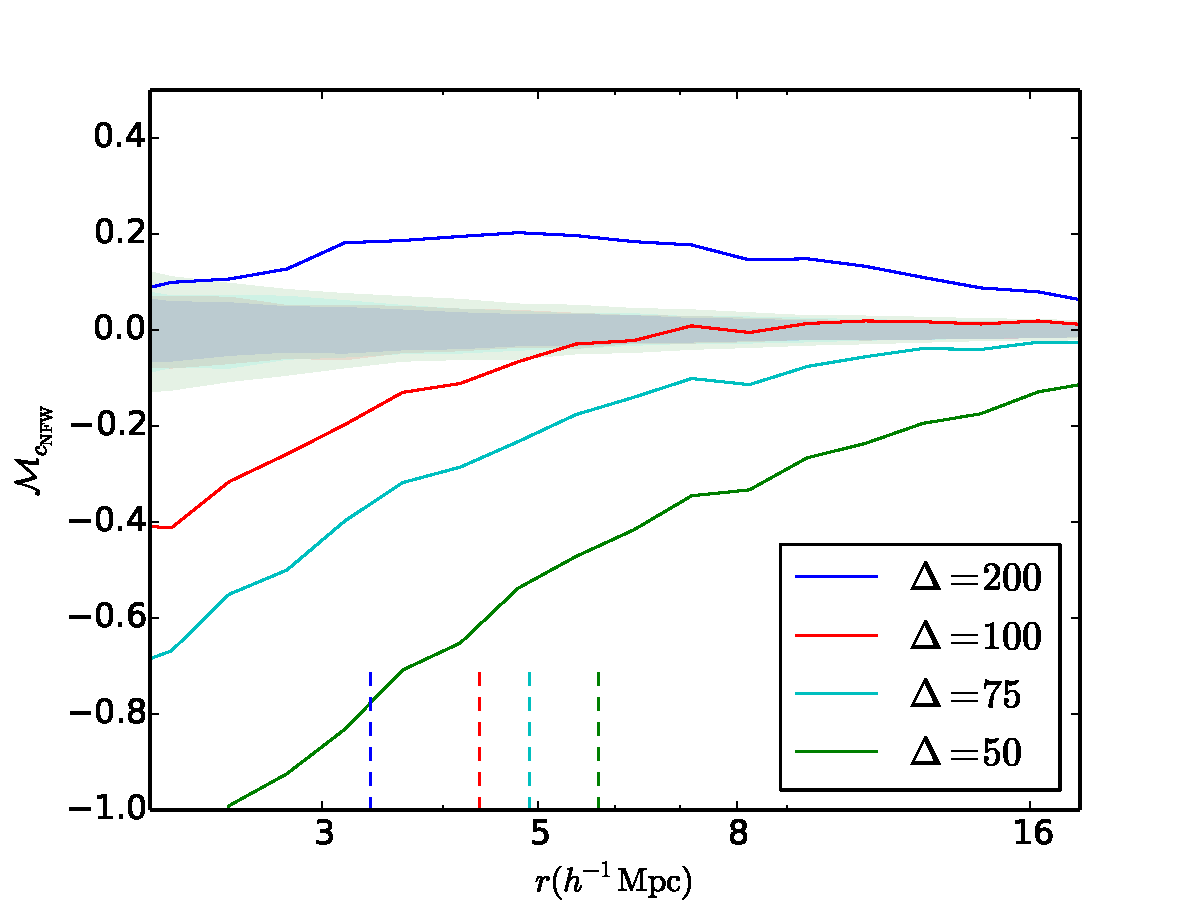
\includegraphics[width=.45\textwidth]{ld_mcf_cnfw_z00_hosts.pdf}} }
	\caption{The marked correlation function for the concentration defined according to the NFW profile. The shaded bands represent 2-sigma confidence regions generated by randomization of the marks. The dashed line denotes the largest halo radius for a given value of the overdensity parameter.}
\end{figure*}

The NFW defined concentration MCF is shown in Figure 4. It can been that as we decrease the value of the overdensity parameter $\Delta$ to lower values down to $\Delta = 50$. It can be seen that at scales of $r > 10 \hMpc$, environmental effects are removed between $\Delta = 100$ and $\Delta =75$. The fact that this holds true over two different realizations and box resolutions seems to indicate that this method is fairly robust.

\begin{figure*}
	\centering
	\subfloat[L0125]{{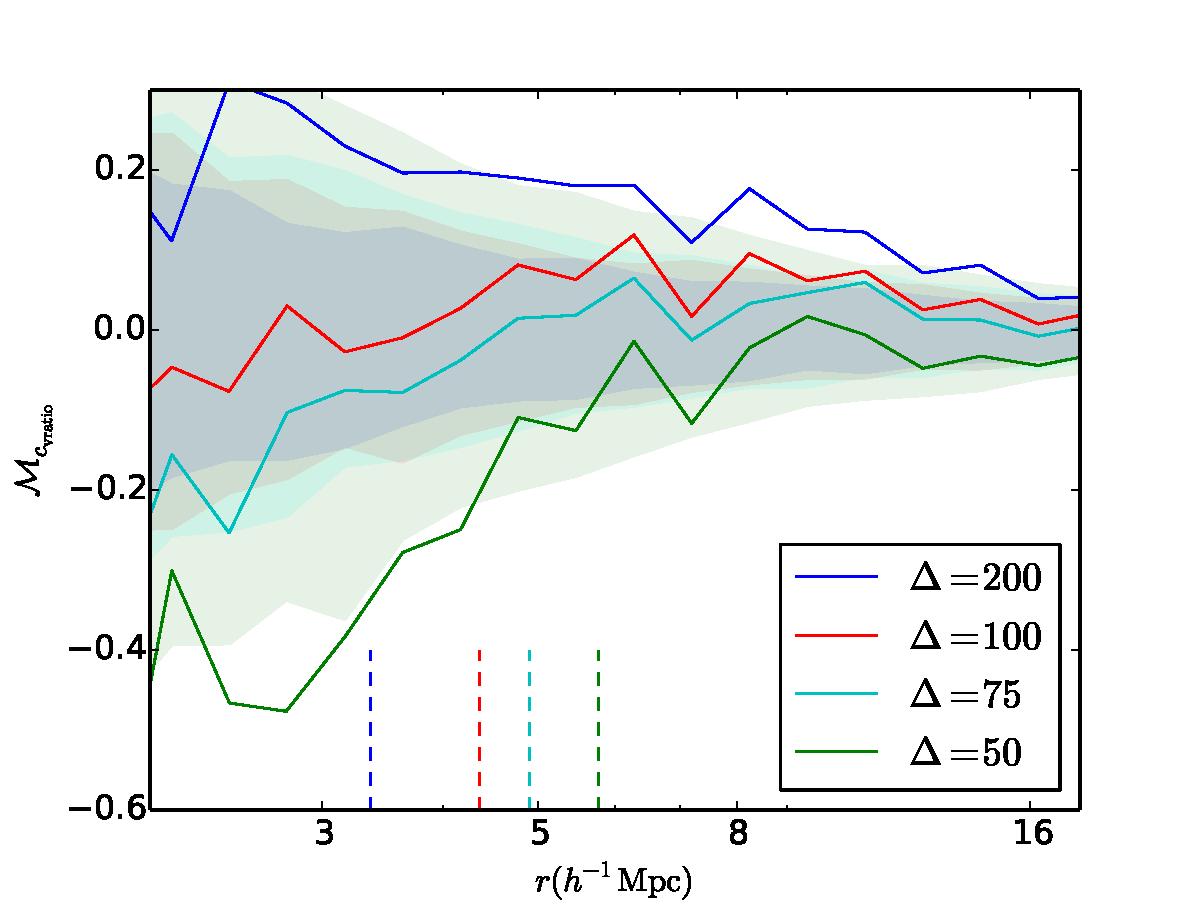
\includegraphics[width=.45\textwidth]{L0125_mcf_vrat_z00_hosts.pdf}} }
	\subfloat[L0250]{{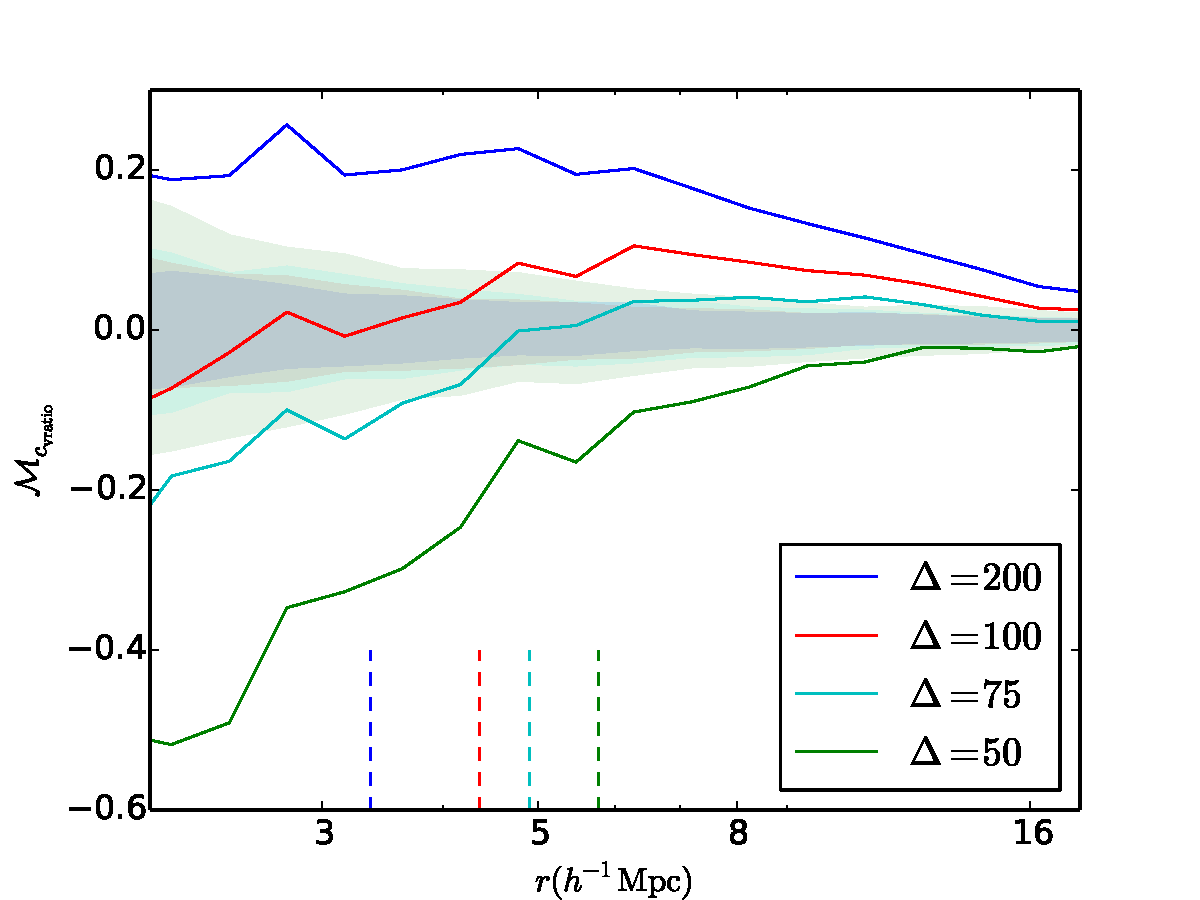
\includegraphics[width=.45\textwidth]{L0250_mcf_vrat_z00_hosts.pdf}} }
	\\
	\subfloat[L0500]{{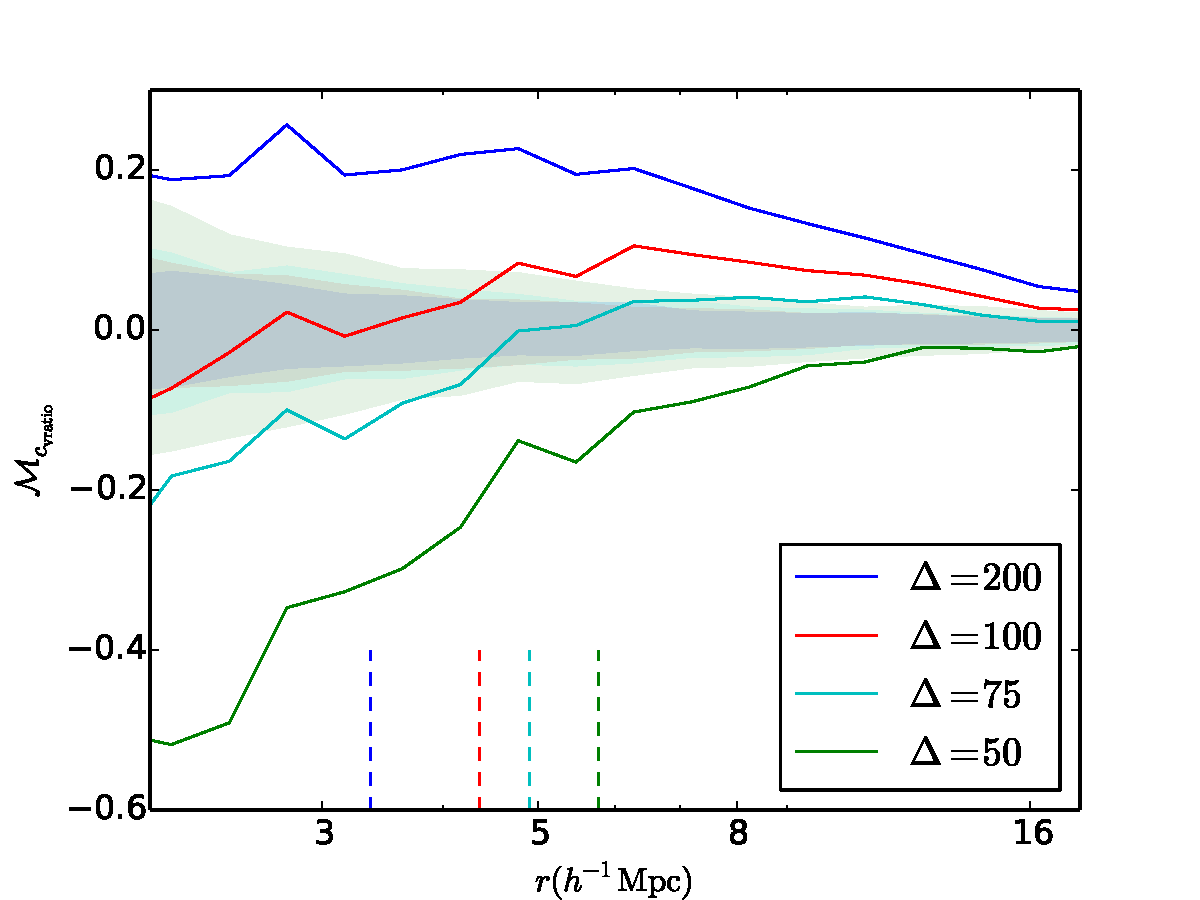
\includegraphics[width=.45\textwidth]{L0250_mcf_vrat_z00_hosts.pdf}} }
	\subfloat[Consuelo]{{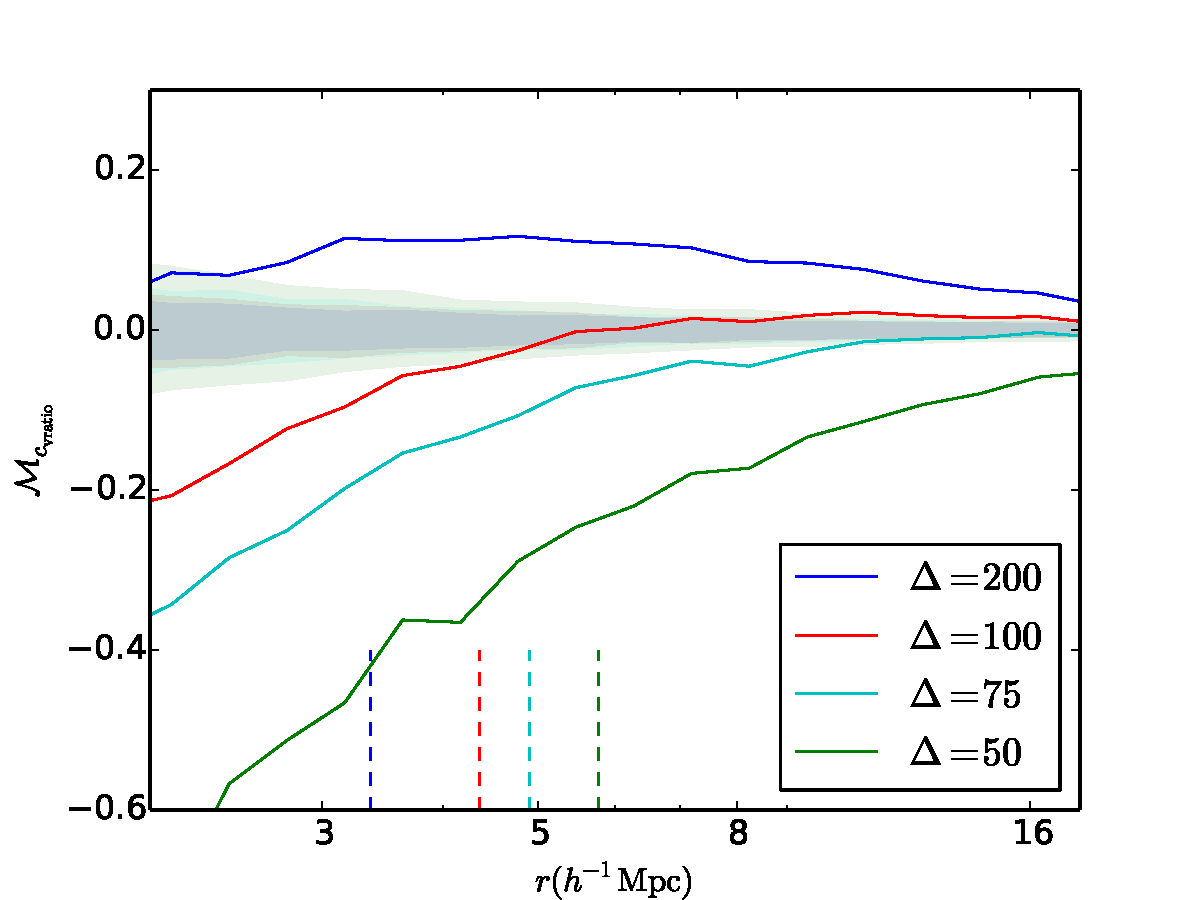
\includegraphics[width=.45\textwidth]{ld_mcf_vrat_z00_hosts.pdf}} }
	\caption{The marked correlation function for the concentration defined according to the velocity ratio. The shaded bands represent 2-sigma confidence regions generated by randomization of the marks. The dashed line denotes the largest halo radius for a given value of the overdensity parameter.}
\end{figure*}

The velocity ratio defined concentration MCF is shown in Figure 5. It can be immediately seen that many of the same features from the previous MCF can be seen in the different concentration proxy. Furthermore, in the range of $\Delta = 100$ and $\Delta=75$, we again see the feature that environmental effects are removed at these large scales. Combined with our previous result, this allows for this halo redefinition to prove useful for studies at this scale with regard to concentration.

\begin{figure*}
	\centering
	\subfloat[L0125]{{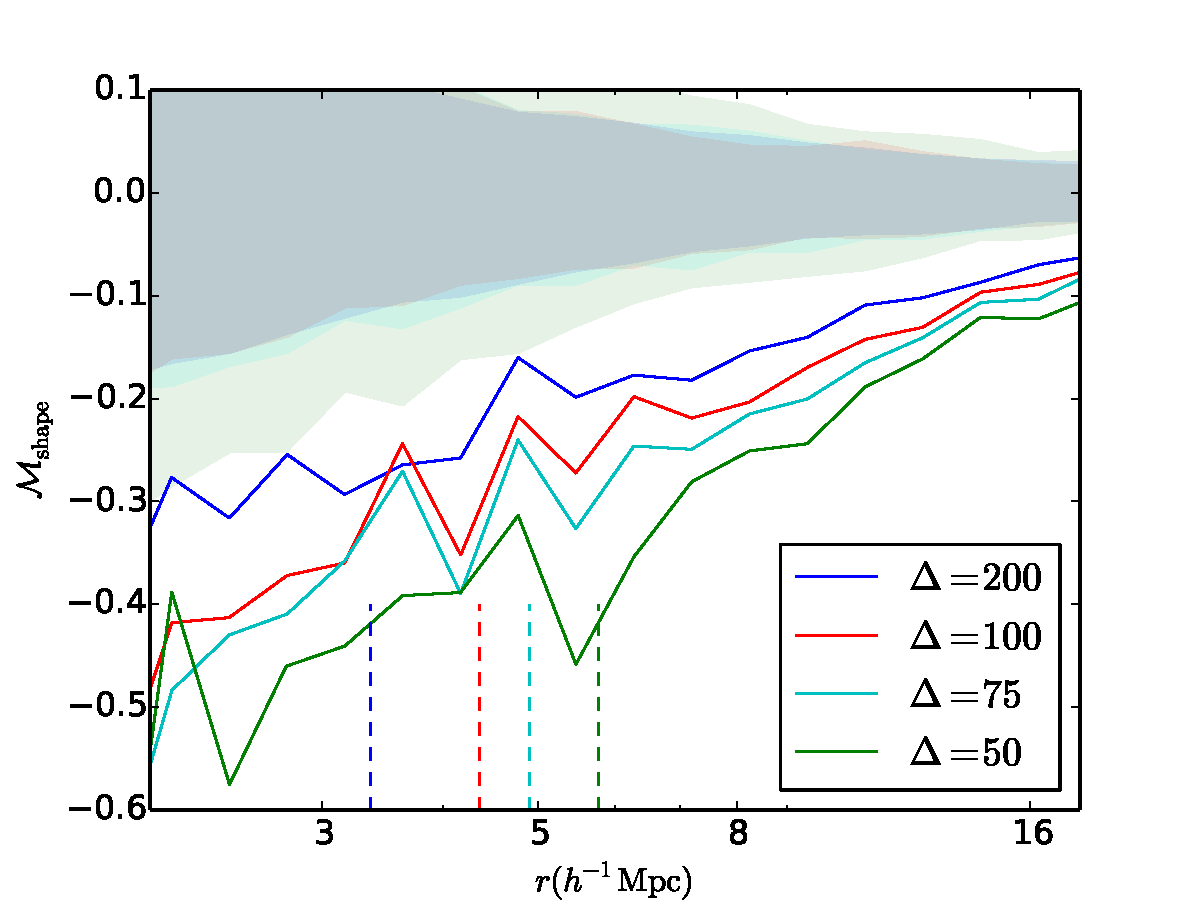
\includegraphics[width=.45\textwidth]{L0125_mcf_s_z00_hosts.pdf}} }
	\subfloat[L0250]{{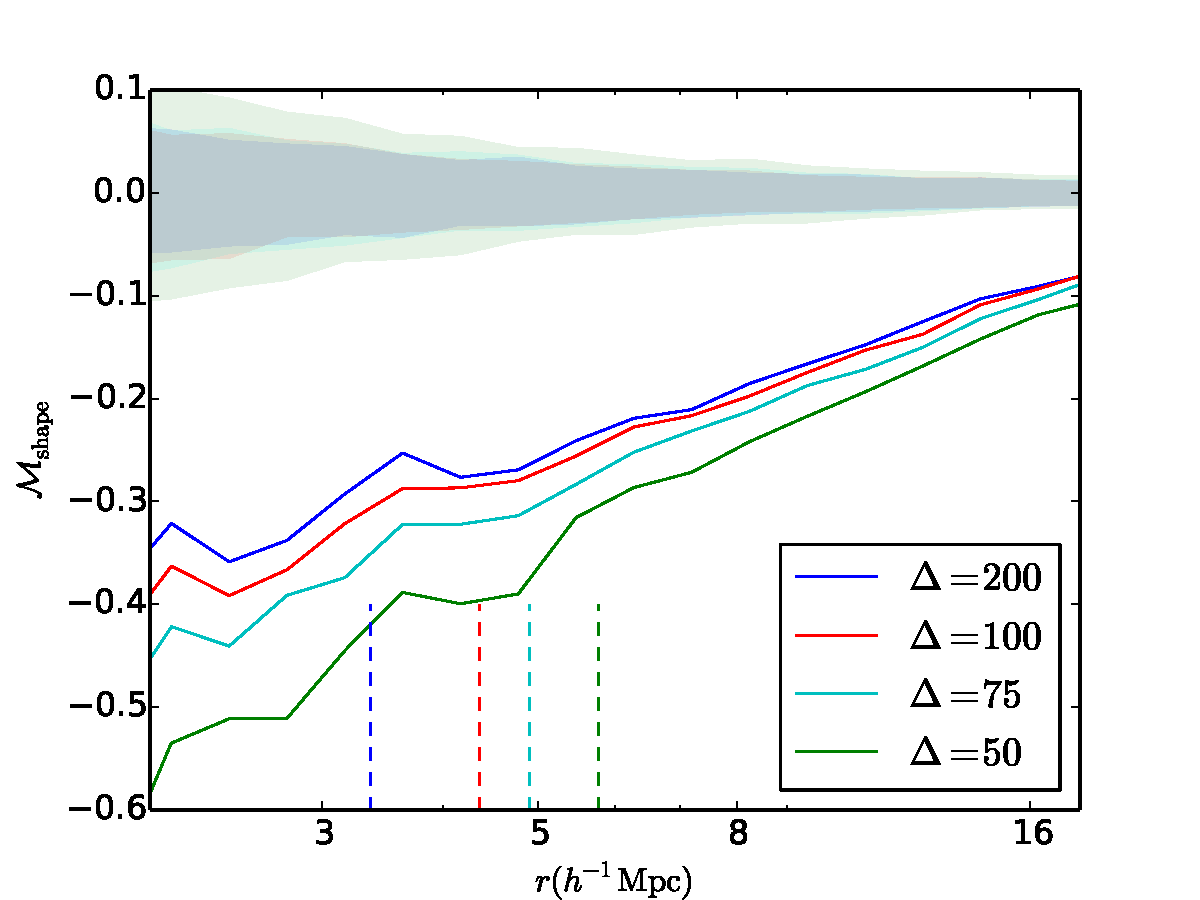
\includegraphics[width=.45\textwidth]{L0250_mcf_s_z00_hosts.pdf}} }
	\\
	\subfloat[L0500]{{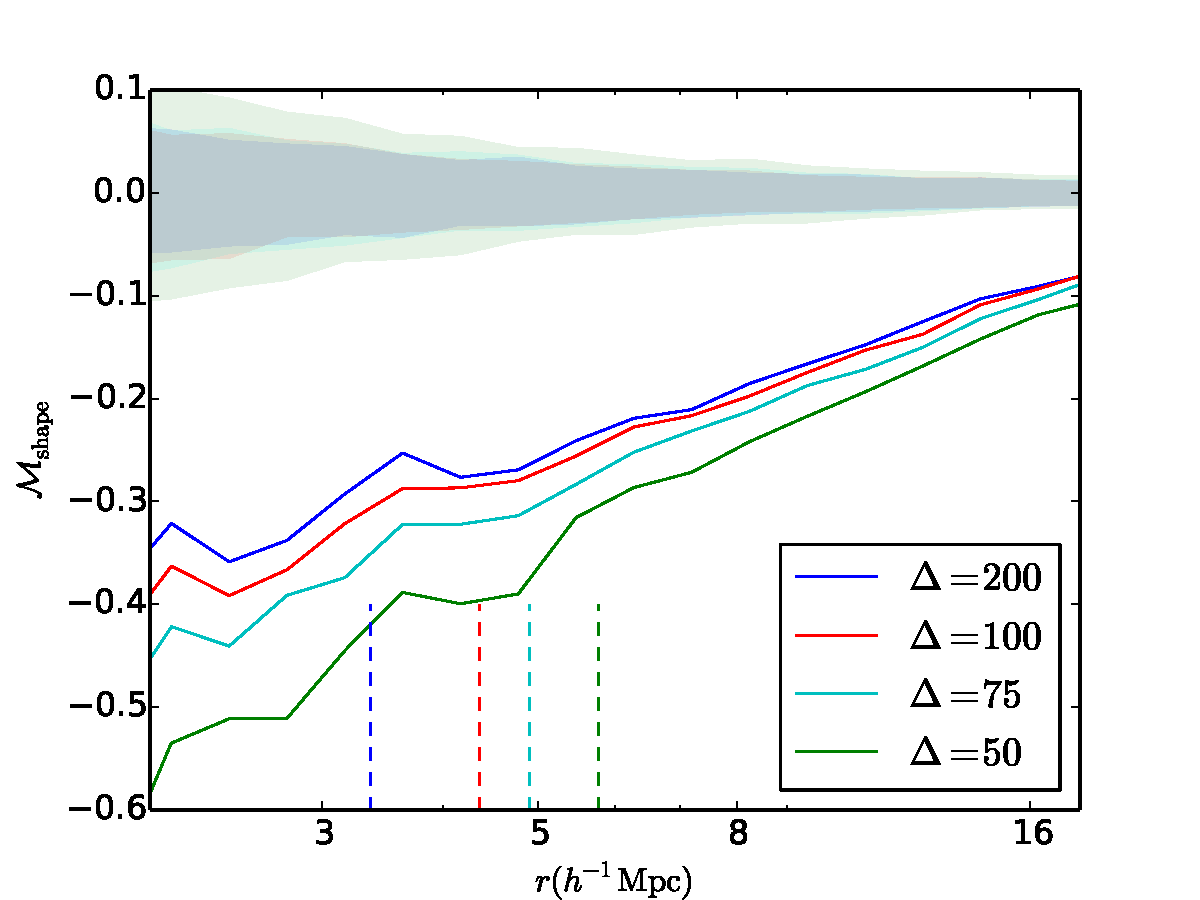
\includegraphics[width=.45\textwidth]{L0250_mcf_s_z00_hosts.pdf}} }
	\subfloat[Consuelo]{{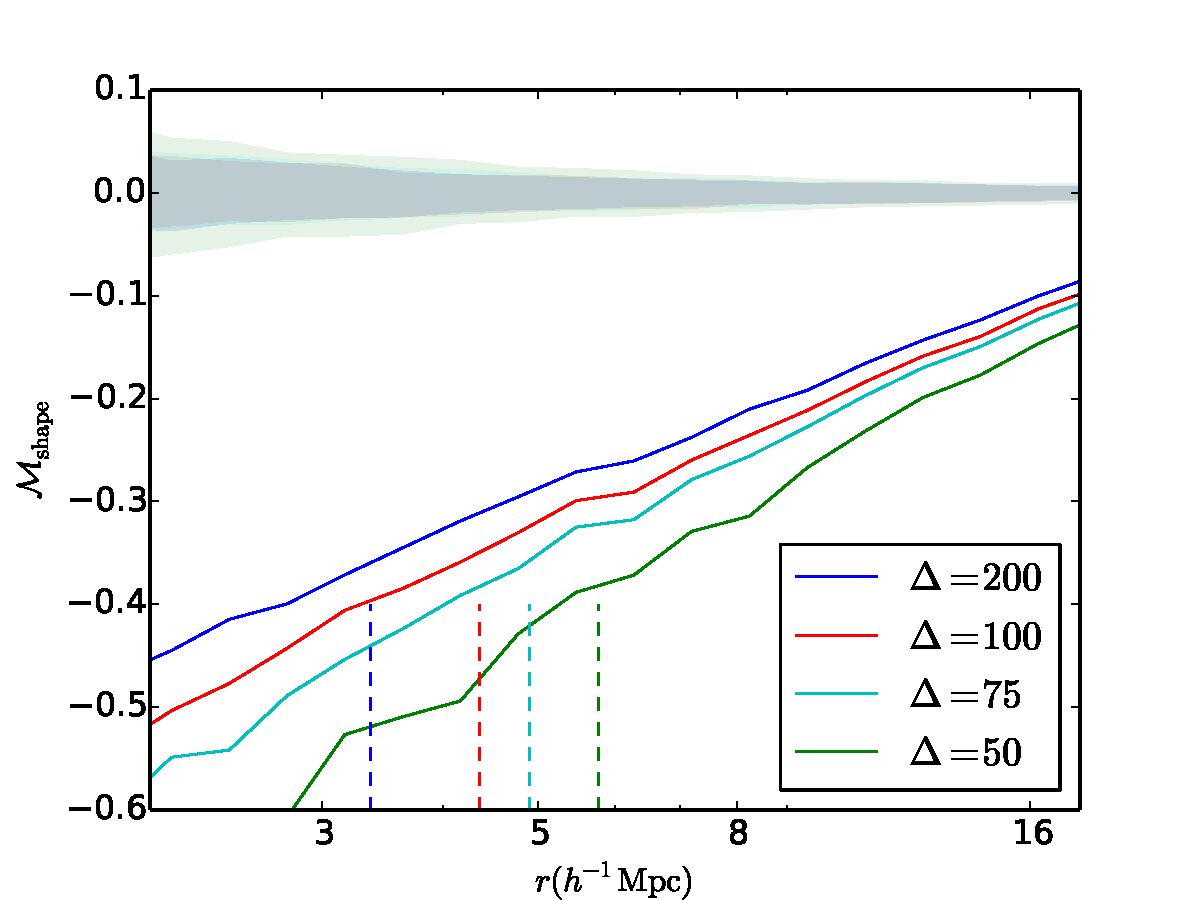
\includegraphics[width=.45\textwidth]{ld_mcf_s_z00_hosts.pdf}} }
	\caption{The marked correlation function for the shape of the halo. The shaded bands represent 2-sigma confidence regions generated by randomization of the marks. The dashed line denotes the largest halo radius for a given value of the overdensity parameter.}
\end{figure*}

Figure 6 demonstrates a case in which the halo property does not have environmental dependence removed under our simple method of halo redefinition. In particular, with decreasing values of $\Delta$, we only serve to increase the strength of this environmental dependence. This result seems to indicate a process occurring to drive the shape of the halo is on scales that are significantly larger than the size of the halo, such that our method will not be able to encompass these effects. A similar result is located in both Figure 7 and Figure 8, in which the spin parameter mark and satellite number mark experience the exact same effect.

\begin{figure*}
	\centering
	\subfloat[L0125]{{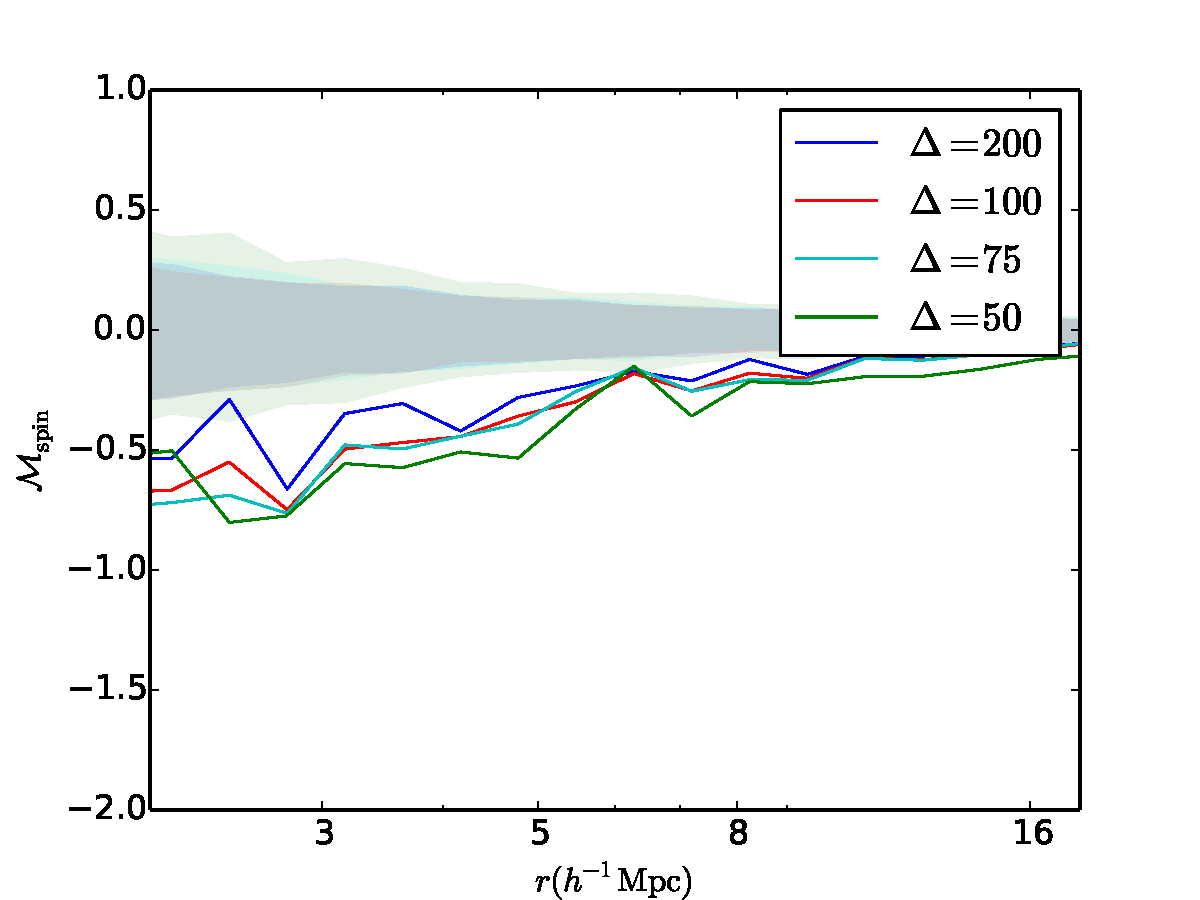
\includegraphics[width=.45\textwidth]{L0125_mcf_spin_z00_hosts.pdf}} }
	\subfloat[L0250]{{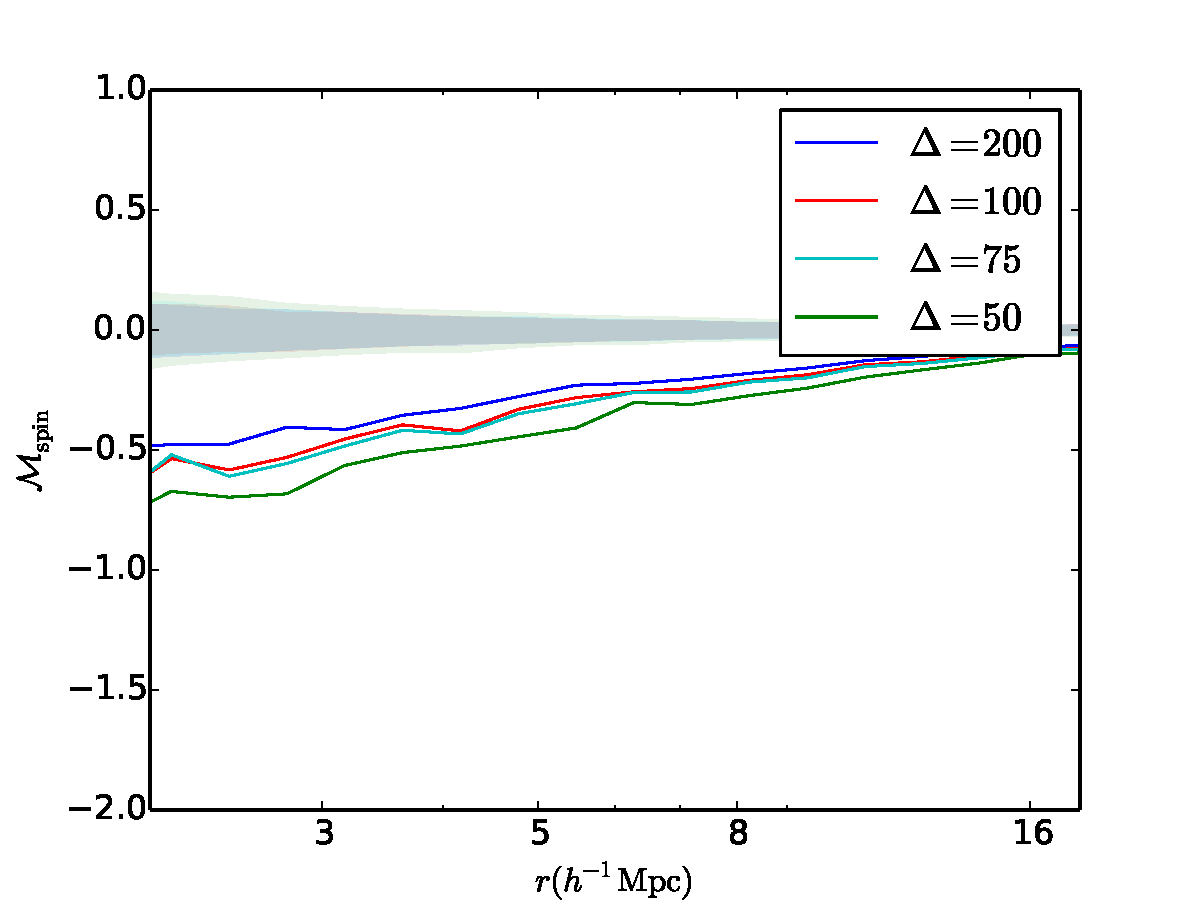
\includegraphics[width=.45\textwidth]{L0250_mcf_spin_z00_hosts.pdf}} }
	\\
	\subfloat[L0500]{{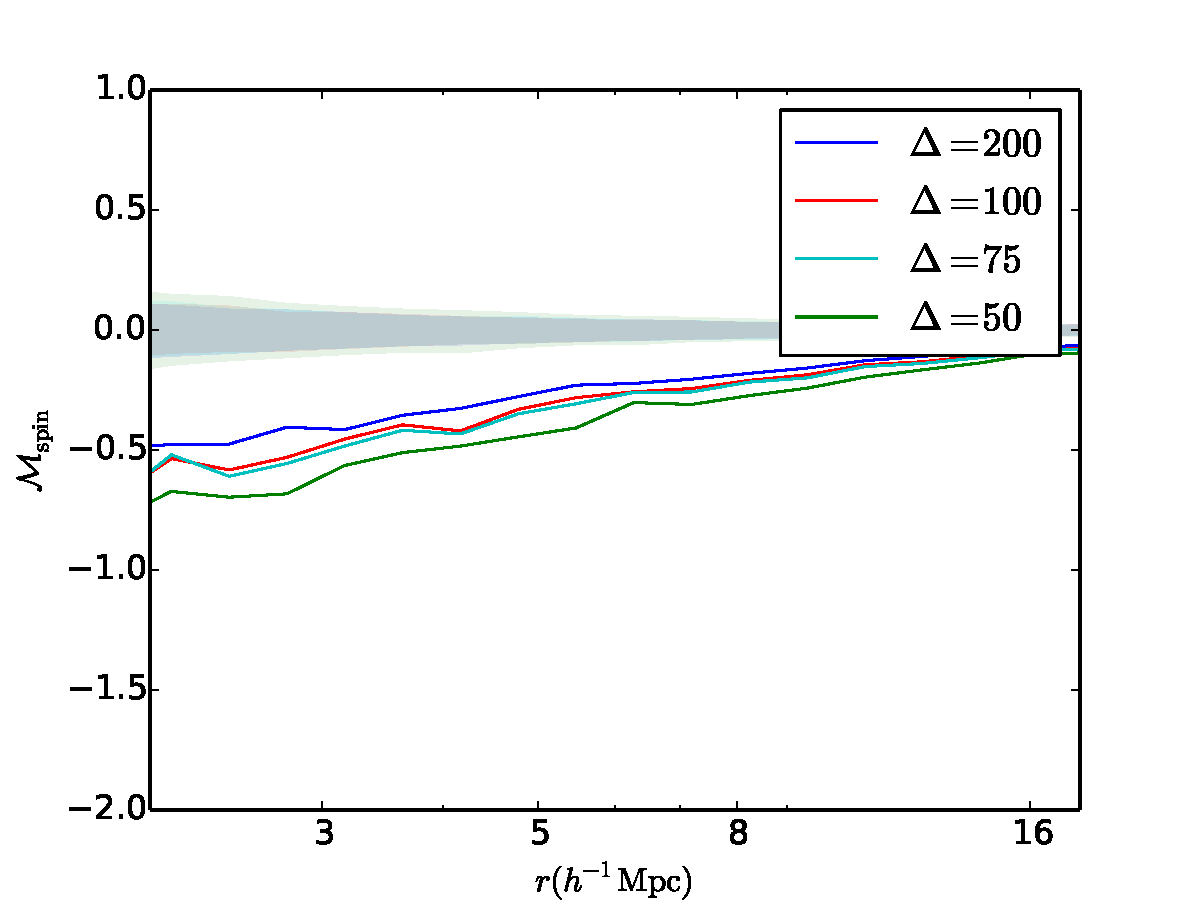
\includegraphics[width=.45\textwidth]{L0250_mcf_spin_z00_hosts.pdf}} }
	\subfloat[Consuelo]{{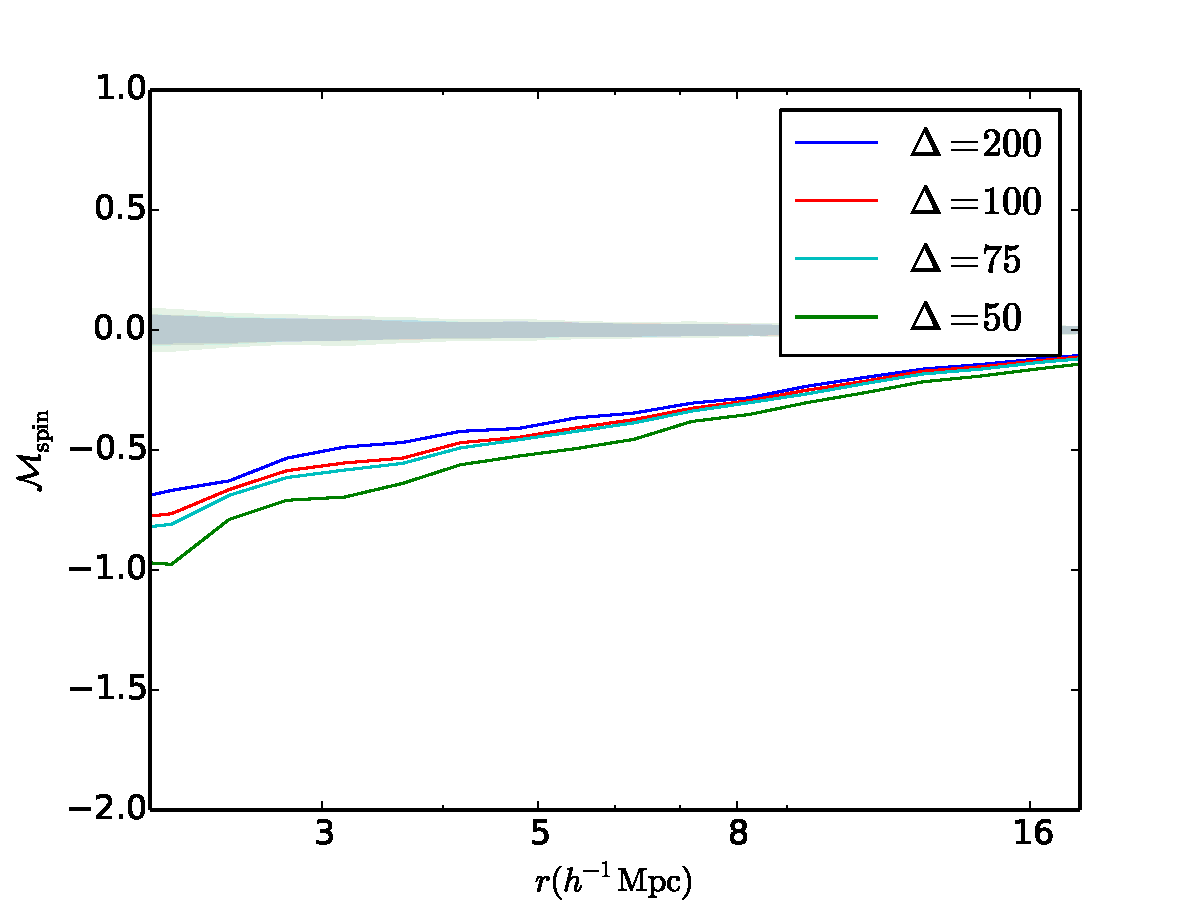
\includegraphics[width=.45\textwidth]{ld_mcf_spin_z00_hosts.pdf}} }
	\caption{The marked correlation function for the spin parameter of the halo. The shaded bands represent 2-sigma confidence regions generated by randomization of the marks. The dashed line denotes the largest halo radius for a given value of the overdensity parameter.}
\end{figure*}

\begin{figure*}
	\centering
	\subfloat[L0125]{{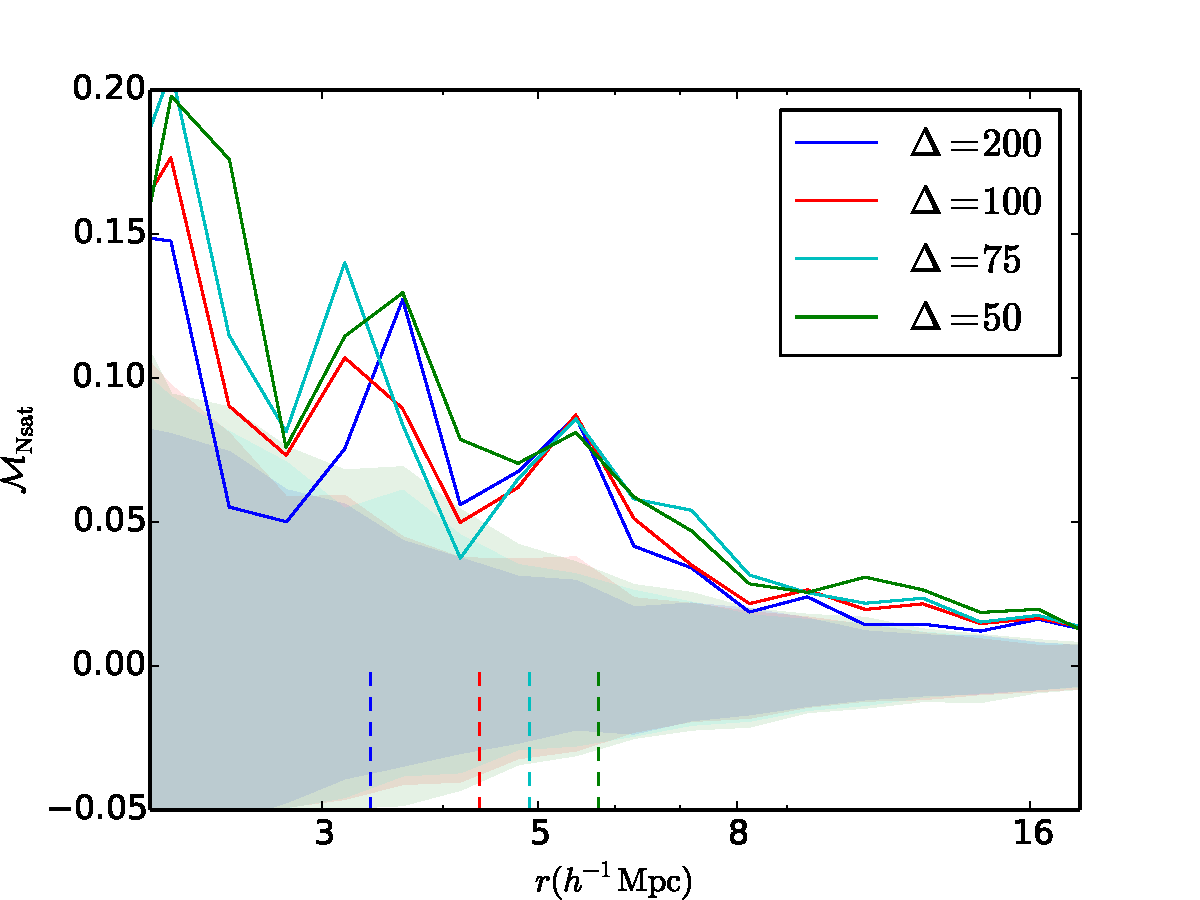
\includegraphics[width=.45\textwidth]{L0125_mcf_ns_z00_hosts.pdf}} }
	\subfloat[L0250]{{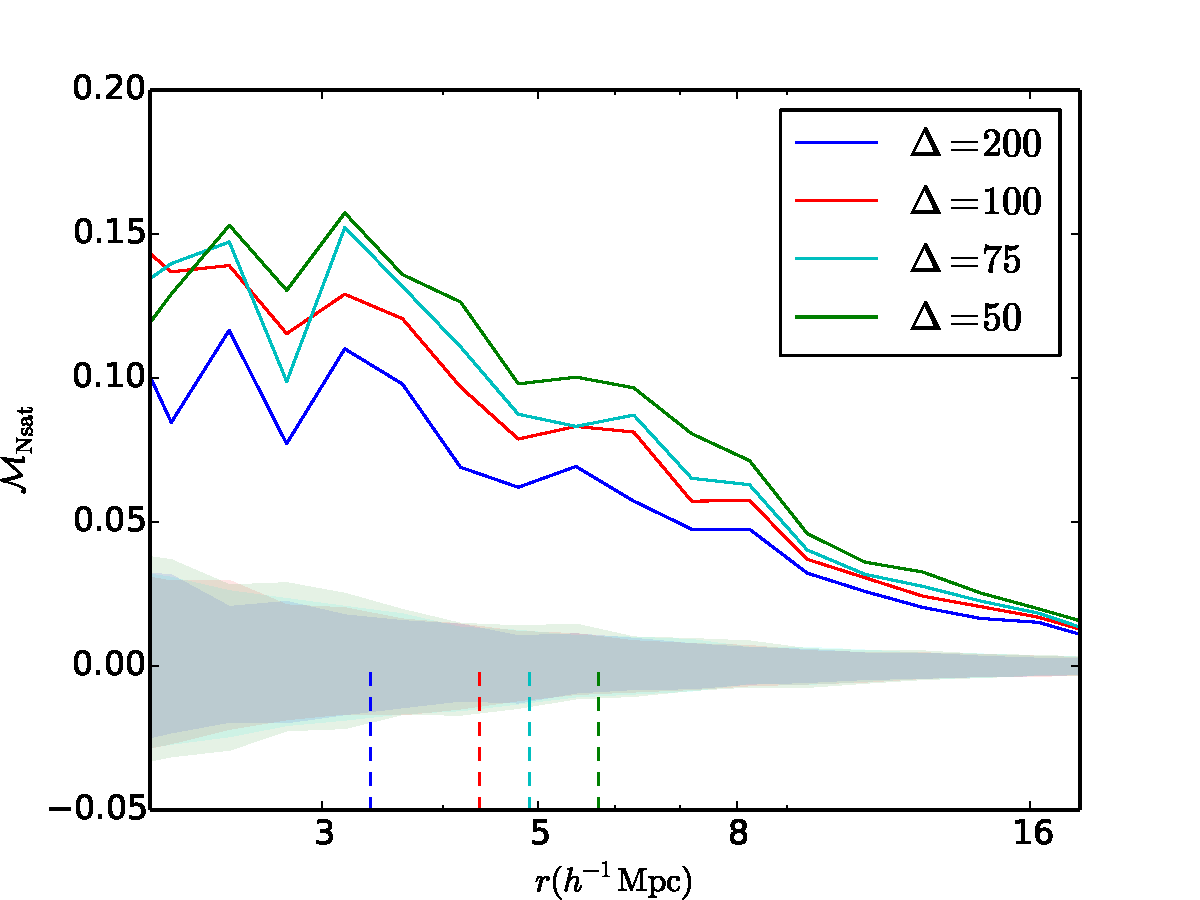
\includegraphics[width=.45\textwidth]{L0250_mcf_ns_z00_hosts.pdf}} }
	\\
	\subfloat[L0500]{{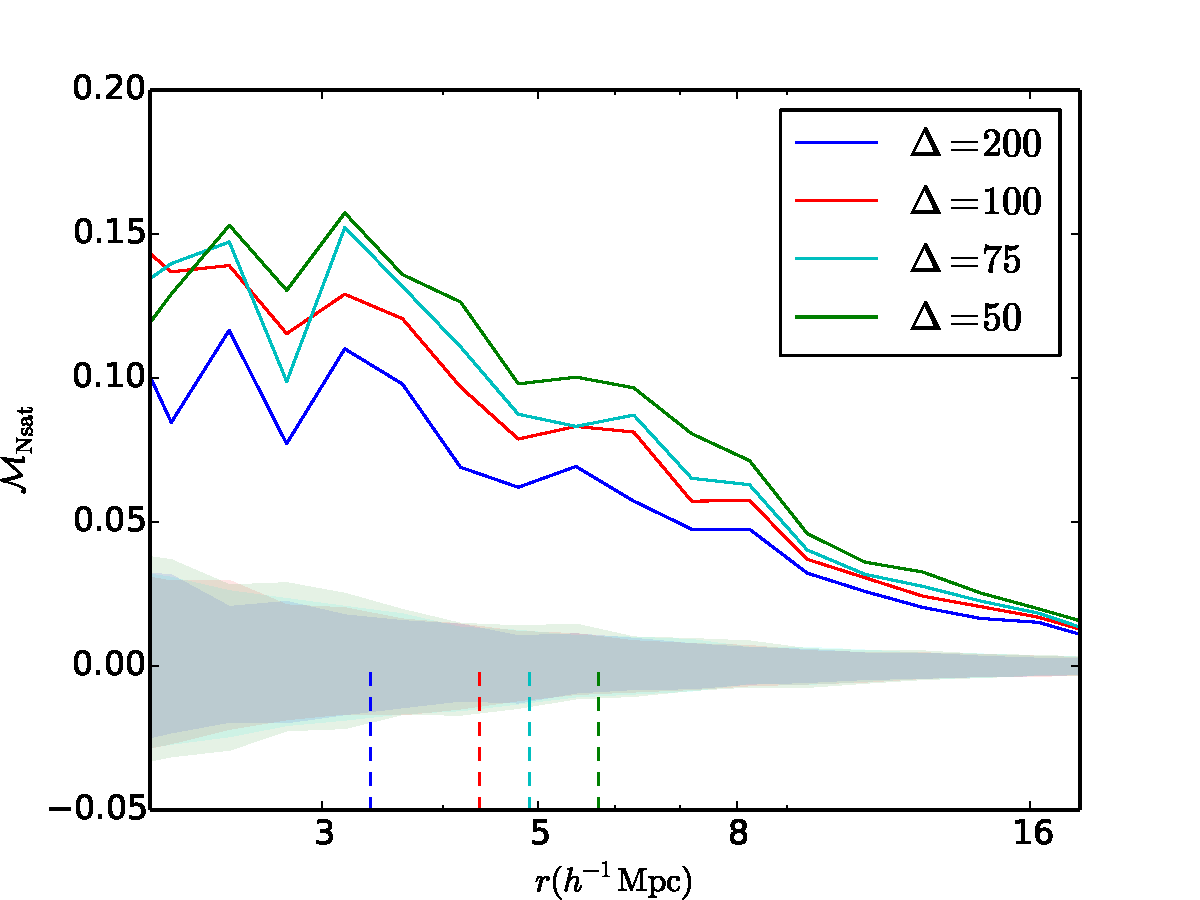
\includegraphics[width=.45\textwidth]{L0250_mcf_ns_z00_hosts.pdf}} }
	\subfloat[Consuelo]{{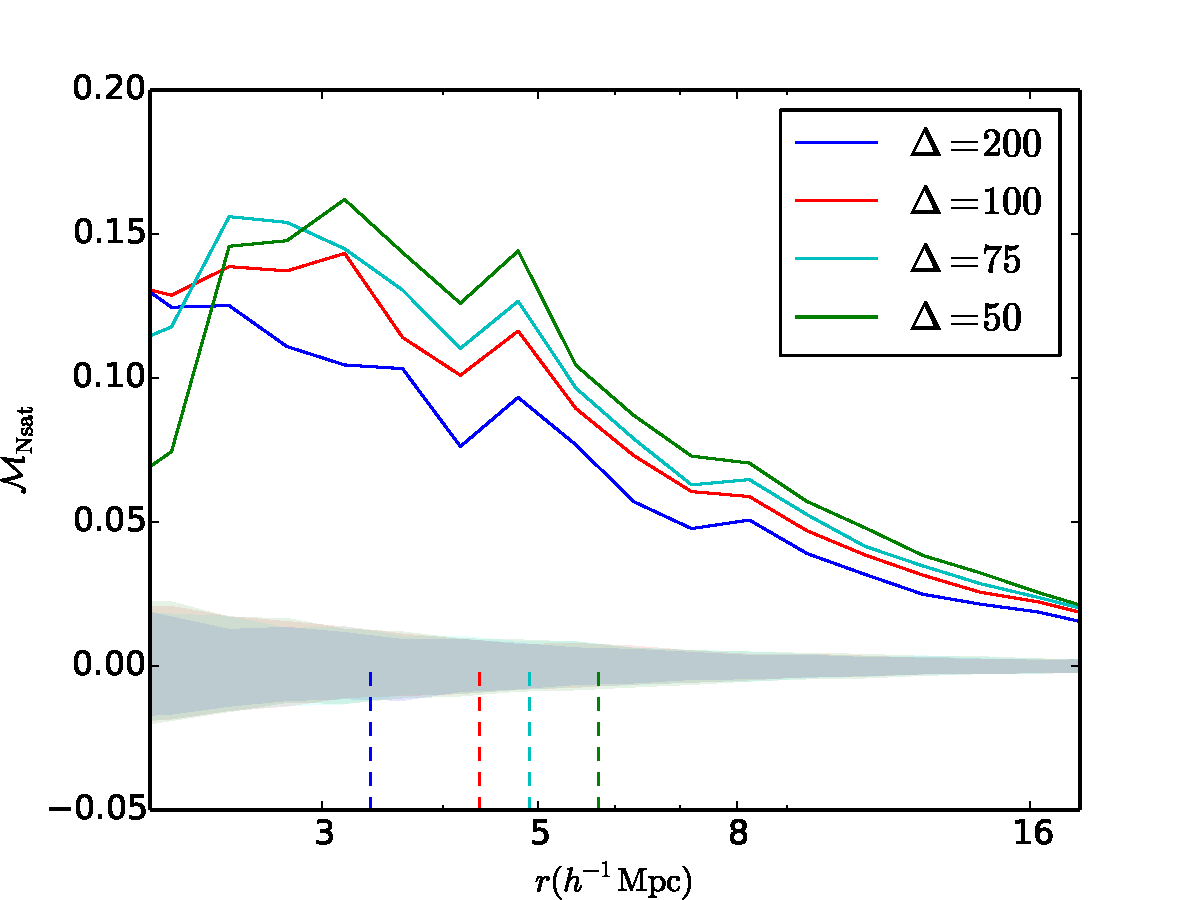
\includegraphics[width=.45\textwidth]{ld_mcf_ns_z00_hosts.pdf}} }
	\caption{The marked correlation function for the satellite number. The shaded bands represent 2-sigma confidence regions generated by randomization of the marks. The dashed line denotes the largest halo radius for a given value of the overdensity parameter.}
\end{figure*}

Overall, while some statistics of the halo can be made to become independent of environmental effects, there exist several that cannot. These environmental effects are not negligible when considering applications of the halo model. In contrast, if one is only interested in the concentration of the halo, it is feasible to take advantage of our methodology in order to remove environmental effects. In contrast, it is not possible to apply the halo model directly to statistics such as the number of satellite halos or the shape without accounting for these environmental effects. We do not yet have a full understanding of what leads to the visible effects that we see on some of these marks, but we present a series of cases in which an intuitive understanding may be gained as to the root causes.

In the case that the halo can be described well by an NFW profile, one expects a direct relationship between the NFW defined halo concentration and the velocity ratio defined halo concentration. While some variation can be expected due to halos not perfectly being fit by an NFW profile, we do see that the features in one concentration proxy are mirrored in the other. This allows for the two concentration markers to support each other well with regards to our ability to remove environmental effects on large scales.

\begin{figure*}
	\centering
	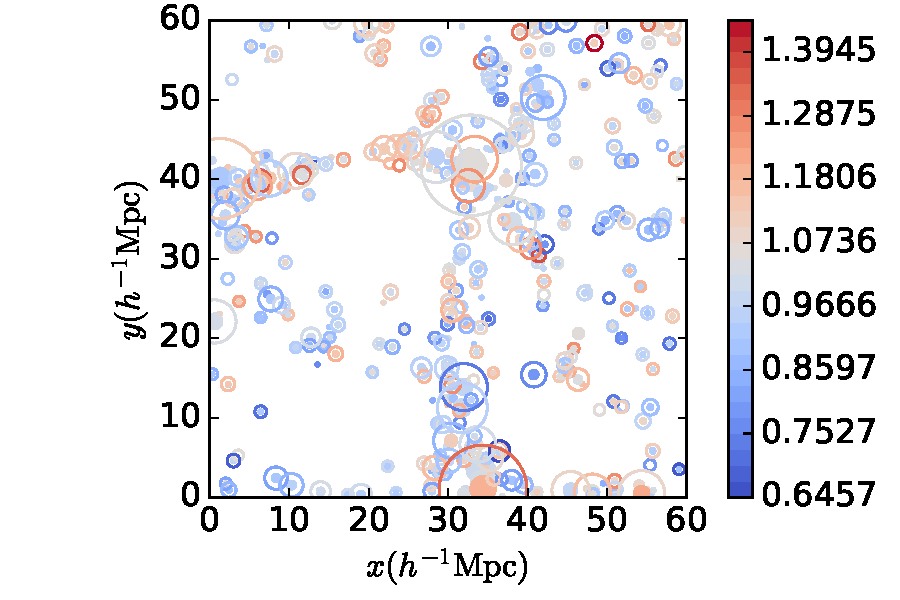
\includegraphics[width=1\textwidth]{plotcircles.pdf}
	\caption{A $5 \hMpc$ deep cut of the Consuelo simulation box along the z-axis. This zoom-in demonstrates the process that decreases the shape parameter as a function of clustering. The size of each circle represents the projection of a spherical dark matter halo with a given halo radius onto the x-y plane. Blue circles use the $\Delta = 200$ catalog and red circles use the $\Delta = 10$ catalog in order to make the effect more visible.}
\end{figure*}

Halo shape and satellite number are statistics that do not end up having their environmental effects removed and can even be made more prominent by our methodology. One intuitive way to consider the former statistic is in the context of the cosmic web. Studies have shown a statistically significant alignment between filaments and satellite galaxy position \citep{tempel15, velliscig15}. Our method then expands the halo radius and subsumes material that was previously outside of the halo. A simple graphic illustrates this potential effect in Figure 8. As there is a preferential distribution of these satellites that are being subsumed into the halo, this would serve to induce a shape to the halo that would then be determined by Rockstar. In addition, as our satellite number is chosen by those halos within the halo radius, we anticipate that the most clustered regions would see the largest increase in satellite count and thus see an increase in the satellite number mark.

The ``sweet spot'' behavior of this method is also of interest to us. The halo redefinition process that we use serves to decrease halo clustering for the most concentrated halos and increase halo clustering for the least concentrated halos. In the case of the high concentration cut, the reduced clustering can be seen as a result of halo exclusion. As we exchange collections of tightly clustered smaller halos for a single larger halo, then the most prominent contribution of the two-point correlation function will be reduced at all scales.


%% add segment examining the mass dependence of this method in particular. Compariosn plots of L0125 vs L0250 and L0250 vs L0500 with the overlapping mass cuts is ideal

%----------------------
\section[]{Conclusions}
\label{section:conclusions}
%----------------------

We have looked at how to use CFs and MCFs in order to analyze the environmental effects upon the properties of the halo. We have suggested a method of removing the mass dependence that is not subject to the small number statistics at large halo masses. Taking our various tests, we then apply a change to the threshold density $\Delta$ in an attempt to remove the effect that environment has upon these properties. We come to the following conclusions from our simulation data.

\begin{itemize}
	\item Our halo redefinition method does not cause any substantial breakdown in the ROCKSTAR halo finding algorithm, though this may not be the case for every halo finding methodology. This is something that should be considered prior to utilization of this method, unless working directly from particle data. As our initial halo sizes and locations are determined through spherical overdensities, it cannot be assumed that starting from a FoF grouping and then determining values through particle data directly will produce identical results. Similarly, different cosmologies may remove environmental effects at different scales.

	\item When looking at the two-point correlation function, there appears to be a ``sweet spot'' that appears to remove environmental effects the most efficiently. Going beyond that seems to reintroduce environmental effects, possibly as an extreme side effect of halo exclusion.

	\item For our marked correlation functions we see that both proxies of concentration that we use as marks show significant removal of environmental effects at large scales for similar values of the overdensity parameter $\Delta$. In cases where one is only interested in the concentration of dark matter halos and large scales (or correspondingly small values of k), this method will allow you to compensate for bias that environment could introduce to calculations dependent upon the halo model. This may prove valuable for calculations such as that of the shear power spectrum calculated through weak lensing.

	\item The environmental effects on the shape of the host halo and the satellite number of the host halo cannot be removed regardless of the chosen redefinition of $\Delta$. We propose that this may be intrinsically tied to the nature of the filaments, whose effects cannot be removed by a simple redefinition of the halo radius.
\end{itemize}

This methodology, while certainly not perfect in removing environmental effects, may be of significance when applied to galaxy formation models. Provided that the properties of interest in a given model behave well under our redefinition, it will allow us to create better mock galaxy catalogs while avoiding the trouble that baryonic physics represent. This may allow us to better study the properties of galaxies within halos without having to substantially increase computation time.

\section*{Acknowledgments}

%%\bibliographystyle{plainnat}
\bibliography{master}

\label{lastpage}

\end{document}
